\section{Frete}

\begin{frame}[fragile]{Problema}

O senhor Satoshi passou anos reclamando da empresa de correios do seu país, porque ela sempre
transportava suas encomendas usando um caminho que passava pelo número mínimo de cidades entre a
cidade onde o senhor Satoshi mora e a cidade destino da encomenda. A empresa alegava que essa
estratégia levava ao menor tempo para a entrega final da encomenda. O problema é que ele notou que
essa estratégia da empresa nem sempre levava ao menor preço para o frete total. Se ele pudesse
escolher o caminho por onde a encomenda deveria passar para ir da sua cidade para a cidade destino,
ele poderia economizar bastante com o frete, já que não havia muita urgência para a maioria de suas
encomendas.

\end{frame}

\begin{frame}[fragile]{Problema}

Depois de muita reclamação, a empresa finalmente está dando aos clientes a opção de determinar o
caminho por onde a encomenda deve passar. O senhor Satoshi, feliz da vida, agora quer a sua ajuda
para implementar um programa que, dado o custo de transporte de uma encomenda entre vários pares de
cidades pelo país, para os quais a empresa realiza entregas diretas, determine qual é o preço total
mínimo para o frete entre a cidade onde ele mora e a cidade destino da encomenda.

\end{frame}

\begin{frame}[fragile]{Problema}

    \begin{figure}[!ht]
        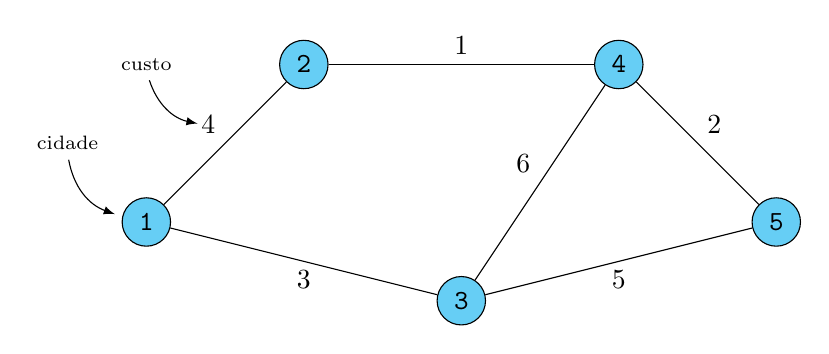
\begin{tikzpicture}
            \node[draw,circle,fill=cyan!60] (A) at (1, 2) { \texttt{1} };
            \node[draw,circle,fill=cyan!60] (B) at (3, 4) { \texttt{2} };
            \node[draw,circle,fill=cyan!60] (C) at (5, 1) { \texttt{3} };
            \node[draw,circle,fill=cyan!60] (D) at (7, 4) { \texttt{4} };
            \node[draw,circle,fill=cyan!60] (E) at (9, 2) { \texttt{5} };
            \node (X) at (0, 3) { \scriptsize cidade };
            \coordinate (Y) at (0.6, 2.1);
            \node (W) at (1, 4) { \scriptsize custo };
            \coordinate (Z) at (1.65, 3.25);

            \draw (A) edge node[anchor=south east] { 4 } (B);
            \draw (A) edge node[anchor=north] { 3 } (C);
            \draw (B) edge node[anchor=south] { 1 } (D);
            \draw (C) edge node[anchor=south east] { 6 } (D);
            \draw (C) edge node[anchor=north] { 5 } (E);
            \draw (D) edge node[anchor=south west] { 2 } (E);
            \draw[-latex] (X) edge[bend right] (Y);
            \draw[-latex] (W) edge[bend right] (Z);
        \end{tikzpicture}
    \end{figure}

\end{frame}

\begin{frame}[fragile]{Problema}

O país tem $N$ cidades, identificadas pelos números de 1 a $N$. O senhor Satoshi mora na cidade 1
e o destino da encomenda será sempre a cidade $N$. É garantido que sempre haverá um caminho de 1
até $N$. No exemplo da figura, para $N=5$, o custo mínimo será 7, para o caminho 1 $\to$ 2 $\to$ 4
$\to$ 5.

\end{frame}

\begin{frame}[fragile]{Entrada e saída}

\textbf{Entrada}

A primeira linha da entrada contém dois números inteiros $N$ e $M$, representando o número de
cidades e quantos pares de cidades possuem entrega direta de encomenda pela empresa. As $M$ linhas
seguintes contêm, cada uma, três inteiros $A, B$ e $C$, indicando que a empresa realiza a entrega
de uma encomenda diretamente entre as cidades $A$ e $B$, cobrando o preço $C$.

\end{frame}

\begin{frame}[fragile]{Entrada e saída}

\textbf{Saída}

Seu programa deve imprimir uma linha contendo um inteiro representando o preço mínimo total para o
frete entre a cidade onde o senhor Satoshi mora, a cidade 1, e a cidade destino da encomenda, a
cidade $N$.

\vspace{0.1in}

\textbf{Restrições}

\begin{itemize}
    \item $2\leq N\leq 100$ e $1\leq M\leq 1000$
    \item $1\leq A, B\leq N$ e $A\neq B$
    \item $1\leq C\leq 1000$
\end{itemize}

\end{frame}

\begin{frame}[fragile]{Exemplo de entradas e saídas}

\begin{minipage}[t]{0.45\textwidth}
\textbf{Entrada}
\begin{verbatim}
5 6
1 2 4
1 3 3
4 3 6
4 5 2
2 4 1
3 5 5
\end{verbatim}
\end{minipage}
\begin{minipage}[t]{0.5\textwidth}
\textbf{Saída}
\begin{verbatim}
7
\end{verbatim}
\end{minipage}
\end{frame}

\begin{frame}[fragile]{Exemplo de entradas e saídas}

\begin{minipage}[t]{0.45\textwidth}
\textbf{Entrada}
\begin{verbatim}
7 10
1 2 5
3 1 32
1 4 3
2 3 4
2 6 20
6 3 1
6 4 9
6 5 6
3 7 18
5 7 2
\end{verbatim}
\end{minipage}
\begin{minipage}[t]{0.5\textwidth}
\textbf{Saída}
\begin{verbatim}
18
\end{verbatim}
\end{minipage}
\end{frame}


\begin{frame}[fragile]{Solução}

    \begin{itemize}
        \item Este é um problema de caminhos mínimos que não requer nenhum tipo de adaptação
            ou interpretação

        \item Este fato, aliado aos limites impostos quanto ao número de vértices e arestas,
            permite a aplicação direta de qualquer algoritmo de caminhos mínimos, sejam algoritmos
            de fonte única (Bellman-Ford ou Dijkstra) ou de múltiplas fontes (Floyd-Warshall)

        \item As diferenças entre estes algoritmos residem na complexidade assintótica de cada um
            e também na simplicidade ou sofisticação da implementação
    \end{itemize}

\end{frame}

\begin{frame}[fragile]{Algoritmo de Bellman-Ford}

    \begin{itemize}
        \item O algoritmo de Bellman-Ford computa o caminho mínimo de todos os vértices de
            um grafo a um nó $s$ dado

        \item Primeiramente ele inicializa a distância de $s$ a $s$ como zero e as demais 
            distâncias como infinito 

        \item A cada iteração, ele visita todas as arestas na tentativa de encurtar um
            caminho já existente por meio da adição de uma nova aresta a este, até que não seja
            mais possível realizar tal redução

        \item A complexidade é $O(NM)$, pois o número máximo de arestas em um caminho mínimo é
            igual a $N - 1$
    \end{itemize}

\end{frame}

\begin{frame}[fragile]{Visualização do algoritmo de Bellman-Ford}

    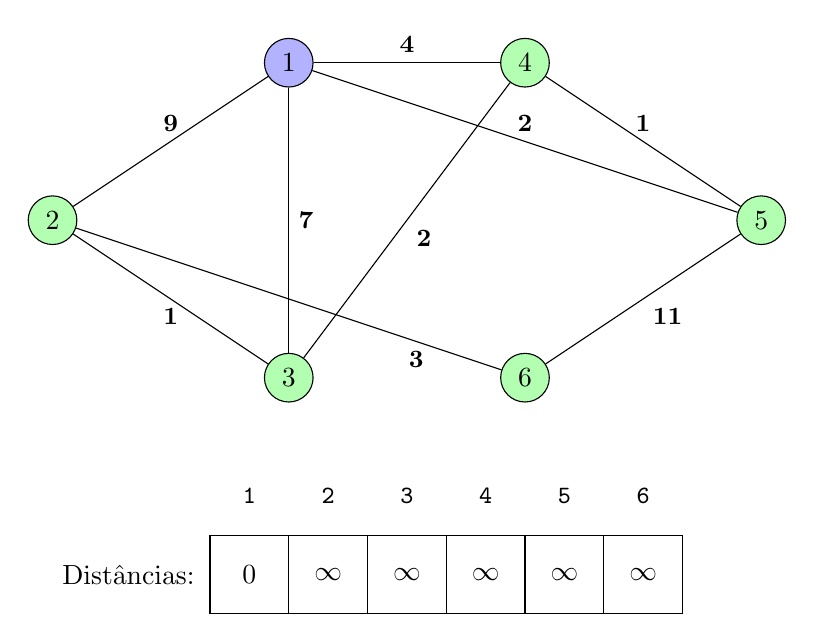
\begin{tikzpicture}
        \node[anchor=west] at (0, 0.5) { Distâncias: };

        \node[circle, draw, fill=blue!30] (a) at (3, 7) {1};
        \node[circle, draw, fill=green!30] (b) at (0, 5) {2};
        \node[circle, draw, fill=green!30] (c) at (3, 3) {3};
        \node[circle, draw, fill=green!30] (d) at (6, 7) {4};
        \node[circle, draw, fill=green!30] (e) at (9, 5) {5};
        \node[circle, draw, fill=green!30] (f) at (6, 3) {6};

        \draw (2, 0) grid (8, 1);

        \node at (2.5, 0.5) { $0$ };
        \node at (3.5, 0.5) { $\infty$ };
        \node at (4.5, 0.5) { $\infty$ };
        \node at (5.5, 0.5) { $\infty$ };
        \node at (6.5, 0.5) { $\infty$ };
        \node at (7.5, 0.5) { $\infty$ };

        \node at (2.5, 1.5) { \small \texttt{1} };
        \node at (3.5, 1.5) { \small \texttt{2} };
        \node at (4.5, 1.5) { \small \texttt{3} };
        \node at (5.5, 1.5) { \small \texttt{4} };
        \node at (6.5, 1.5) { \small \texttt{5} };
        \node at (7.5, 1.5) { \small \texttt{6} };

        \draw (a) to node[midway,anchor=south] { \small \bfseries 9 } (b);
        \draw (a) to node[midway,anchor=west] { \small \bfseries 7 } (c);
        \draw (a) to node[midway,anchor=south] { \small \bfseries 4 } (d);
        \draw (a) to node[midway,anchor=south] { \small \bfseries 2 } (e);
        \draw (b) to node[midway,anchor=north] { \small \bfseries 1 } (c);
        \draw (b) to node[pos=0.8,anchor=north] { \small \bfseries 3 } (f);
        \draw (c) to node[midway,anchor=north west] { \small \bfseries 2 } (d);
        \draw (d) to node[midway,anchor=south] { \small \bfseries 1 } (e);
        \draw (e) to node[midway,anchor=north west] { \small \bfseries 11 } (f);

    \end{tikzpicture}

\end{frame}

\begin{frame}[fragile]{Visualização do algoritmo de Bellman-Ford}

    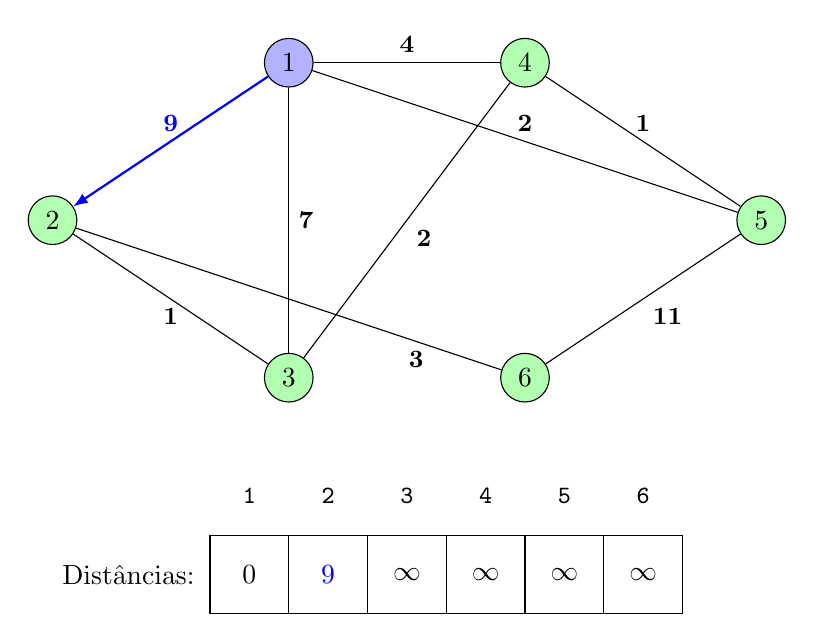
\begin{tikzpicture}
        \node[anchor=west] at (0, 0.5) { Distâncias: };

        \node[circle, draw, fill=blue!30] (a) at (3, 7) {1};
        \node[circle, draw, fill=green!30] (b) at (0, 5) {2};
        \node[circle, draw, fill=green!30] (c) at (3, 3) {3};
        \node[circle, draw, fill=green!30] (d) at (6, 7) {4};
        \node[circle, draw, fill=green!30] (e) at (9, 5) {5};
        \node[circle, draw, fill=green!30] (f) at (6, 3) {6};

        \draw (2, 0) grid (8, 1);

        \node at (2.5, 0.5) { $0$ };
        \node at (3.5, 0.5) { \textcolor{blue}{$9$} };
        \node at (4.5, 0.5) { $\infty$ };
        \node at (5.5, 0.5) { $\infty$ };
        \node at (6.5, 0.5) { $\infty$ };
        \node at (7.5, 0.5) { $\infty$ };

        \node at (2.5, 1.5) { \small \texttt{1} };
        \node at (3.5, 1.5) { \small \texttt{2} };
        \node at (4.5, 1.5) { \small \texttt{3} };
        \node at (5.5, 1.5) { \small \texttt{4} };
        \node at (6.5, 1.5) { \small \texttt{5} };
        \node at (7.5, 1.5) { \small \texttt{6} };

        \draw[-latex,thick,blue] (a) to node[midway,anchor=south] { \small \bfseries 9 } (b);
        %\draw (a) to node[midway,anchor=south] { \small \bfseries 9 } (b);
        \draw (a) to node[midway,anchor=west] { \small \bfseries 7 } (c);
        \draw (a) to node[midway,anchor=south] { \small \bfseries 4 } (d);
        \draw (a) to node[midway,anchor=south] { \small \bfseries 2 } (e);
        \draw (b) to node[midway,anchor=north] { \small \bfseries 1 } (c);
        \draw (b) to node[pos=0.8,anchor=north] { \small \bfseries 3 } (f);
        \draw (c) to node[midway,anchor=north west] { \small \bfseries 2 } (d);
        \draw (d) to node[midway,anchor=south] { \small \bfseries 1 } (e);
        \draw (e) to node[midway,anchor=north west] { \small \bfseries 11 } (f);

    \end{tikzpicture}

\end{frame}

\begin{frame}[fragile]{Visualização do algoritmo de Bellman-Ford}

    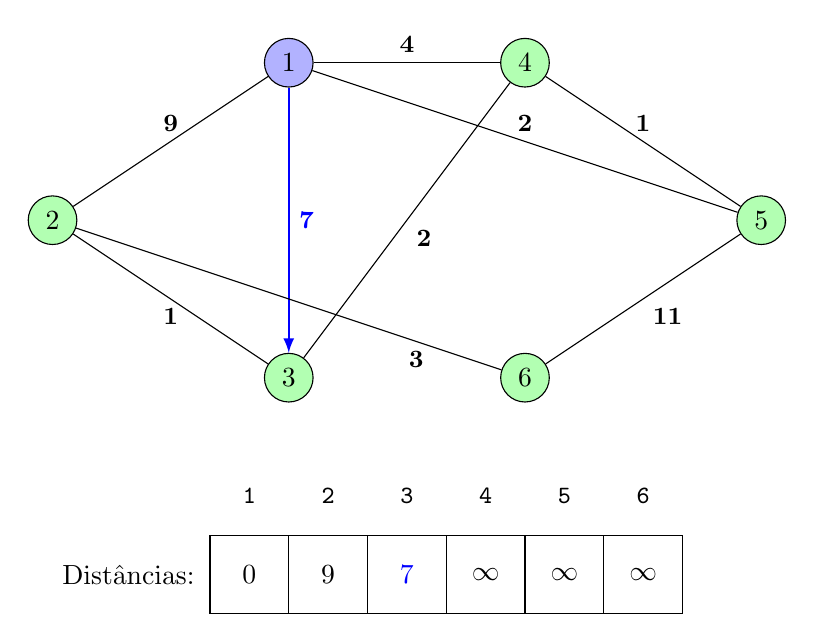
\begin{tikzpicture}
        \node[anchor=west] at (0, 0.5) { Distâncias: };

        \node[circle, draw, fill=blue!30] (a) at (3, 7) {1};
        \node[circle, draw, fill=green!30] (b) at (0, 5) {2};
        \node[circle, draw, fill=green!30] (c) at (3, 3) {3};
        \node[circle, draw, fill=green!30] (d) at (6, 7) {4};
        \node[circle, draw, fill=green!30] (e) at (9, 5) {5};
        \node[circle, draw, fill=green!30] (f) at (6, 3) {6};

        \draw (2, 0) grid (8, 1);

        \node at (2.5, 0.5) { $0$ };
        \node at (3.5, 0.5) { \textcolor{black}{$9$} };
        \node at (4.5, 0.5) { \textcolor{blue}{$7$} };
        \node at (5.5, 0.5) { $\infty$ };
        \node at (6.5, 0.5) { $\infty$ };
        \node at (7.5, 0.5) { $\infty$ };

        \node at (2.5, 1.5) { \small \texttt{1} };
        \node at (3.5, 1.5) { \small \texttt{2} };
        \node at (4.5, 1.5) { \small \texttt{3} };
        \node at (5.5, 1.5) { \small \texttt{4} };
        \node at (6.5, 1.5) { \small \texttt{5} };
        \node at (7.5, 1.5) { \small \texttt{6} };

        \draw (a) to node[midway,anchor=south] { \small \bfseries 9 } (b);
        %\draw (a) to node[midway,anchor=west] { \small \bfseries 7 } (c);
        \draw[-latex,thick,blue] (a) to node[midway,anchor=west] { \small \bfseries 7 } (c);
        \draw (a) to node[midway,anchor=south] { \small \bfseries 4 } (d);
        \draw (a) to node[midway,anchor=south] { \small \bfseries 2 } (e);
        \draw (b) to node[midway,anchor=north] { \small \bfseries 1 } (c);
        \draw (b) to node[pos=0.8,anchor=north] { \small \bfseries 3 } (f);
        \draw (c) to node[midway,anchor=north west] { \small \bfseries 2 } (d);
        \draw (d) to node[midway,anchor=south] { \small \bfseries 1 } (e);
        \draw (e) to node[midway,anchor=north west] { \small \bfseries 11 } (f);

    \end{tikzpicture}

\end{frame}

\begin{frame}[fragile]{Visualização do algoritmo de Bellman-Ford}

    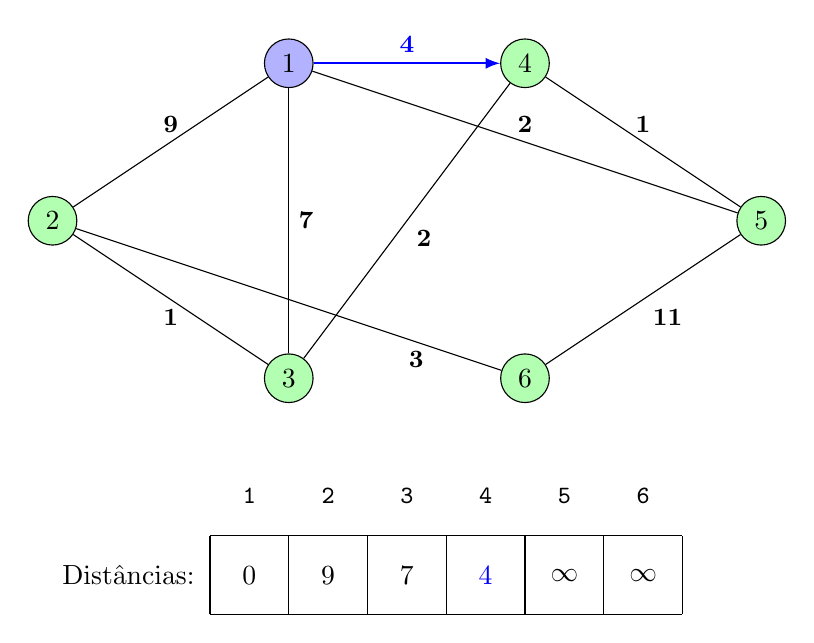
\begin{tikzpicture}
        \node[anchor=west] at (0, 0.5) { Distâncias: };

        \node[circle, draw, fill=blue!30] (a) at (3, 7) {1};
        \node[circle, draw, fill=green!30] (b) at (0, 5) {2};
        \node[circle, draw, fill=green!30] (c) at (3, 3) {3};
        \node[circle, draw, fill=green!30] (d) at (6, 7) {4};
        \node[circle, draw, fill=green!30] (e) at (9, 5) {5};
        \node[circle, draw, fill=green!30] (f) at (6, 3) {6};

        \draw (2, 0) grid (8, 1);

        \node at (2.5, 0.5) { $0$ };
        \node at (3.5, 0.5) { \textcolor{black}{$9$} };
        \node at (4.5, 0.5) { \textcolor{black}{$7$} };
        \node at (5.5, 0.5) { \textcolor{blue}{$4$} };
        \node at (6.5, 0.5) { $\infty$ };
        \node at (7.5, 0.5) { $\infty$ };

        \node at (2.5, 1.5) { \small \texttt{1} };
        \node at (3.5, 1.5) { \small \texttt{2} };
        \node at (4.5, 1.5) { \small \texttt{3} };
        \node at (5.5, 1.5) { \small \texttt{4} };
        \node at (6.5, 1.5) { \small \texttt{5} };
        \node at (7.5, 1.5) { \small \texttt{6} };

        \draw (a) to node[midway,anchor=south] { \small \bfseries 9 } (b);
        \draw (a) to node[midway,anchor=west] { \small \bfseries 7 } (c);
        %\draw (a) to node[midway,anchor=south] { \small \bfseries 4 } (d);
        \draw[-latex,thick,blue] (a) to node[midway,anchor=south] { \small \bfseries 4 } (d);
        \draw (a) to node[midway,anchor=south] { \small \bfseries 2 } (e);
        \draw (b) to node[midway,anchor=north] { \small \bfseries 1 } (c);
        \draw (b) to node[pos=0.8,anchor=north] { \small \bfseries 3 } (f);
        \draw (c) to node[midway,anchor=north west] { \small \bfseries 2 } (d);
        \draw (d) to node[midway,anchor=south] { \small \bfseries 1 } (e);
        \draw (e) to node[midway,anchor=north west] { \small \bfseries 11 } (f);

    \end{tikzpicture}

\end{frame}

\begin{frame}[fragile]{Visualização do algoritmo de Bellman-Ford}

    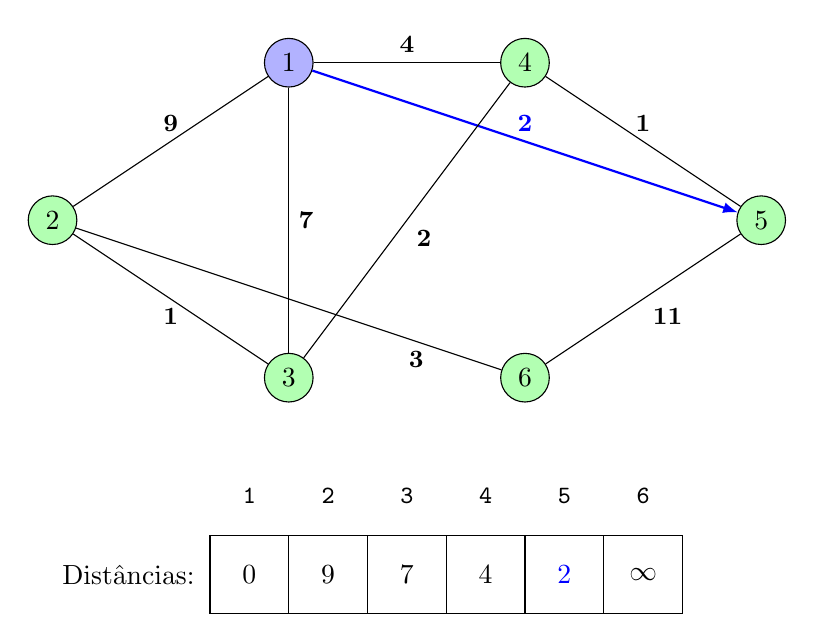
\begin{tikzpicture}
        \node[anchor=west] at (0, 0.5) { Distâncias: };

        \node[circle, draw, fill=blue!30] (a) at (3, 7) {1};
        \node[circle, draw, fill=green!30] (b) at (0, 5) {2};
        \node[circle, draw, fill=green!30] (c) at (3, 3) {3};
        \node[circle, draw, fill=green!30] (d) at (6, 7) {4};
        \node[circle, draw, fill=green!30] (e) at (9, 5) {5};
        \node[circle, draw, fill=green!30] (f) at (6, 3) {6};

        \draw (2, 0) grid (8, 1);

        \node at (2.5, 0.5) { $0$ };
        \node at (3.5, 0.5) { \textcolor{black}{$9$} };
        \node at (4.5, 0.5) { \textcolor{black}{$7$} };
        \node at (5.5, 0.5) { \textcolor{black}{$4$} };
        \node at (6.5, 0.5) { \textcolor{blue}{$2$} };
        \node at (7.5, 0.5) { $\infty$ };

        \node at (2.5, 1.5) { \small \texttt{1} };
        \node at (3.5, 1.5) { \small \texttt{2} };
        \node at (4.5, 1.5) { \small \texttt{3} };
        \node at (5.5, 1.5) { \small \texttt{4} };
        \node at (6.5, 1.5) { \small \texttt{5} };
        \node at (7.5, 1.5) { \small \texttt{6} };

        \draw (a) to node[midway,anchor=south] { \small \bfseries 9 } (b);
        \draw (a) to node[midway,anchor=west] { \small \bfseries 7 } (c);
        \draw (a) to node[midway,anchor=south] { \small \bfseries 4 } (d);
        %\draw (a) to node[midway,anchor=south] { \small \bfseries 2 } (e);
        \draw[-latex,thick,blue] (a) to node[midway,anchor=south] { \small \bfseries 2 } (e);
        \draw (b) to node[midway,anchor=north] { \small \bfseries 1 } (c);
        \draw (b) to node[pos=0.8,anchor=north] { \small \bfseries 3 } (f);
        \draw (c) to node[midway,anchor=north west] { \small \bfseries 2 } (d);
        \draw (d) to node[midway,anchor=south] { \small \bfseries 1 } (e);
        \draw (e) to node[midway,anchor=north west] { \small \bfseries 11 } (f);

    \end{tikzpicture}

\end{frame}

\begin{frame}[fragile]{Visualização do algoritmo de Bellman-Ford}

    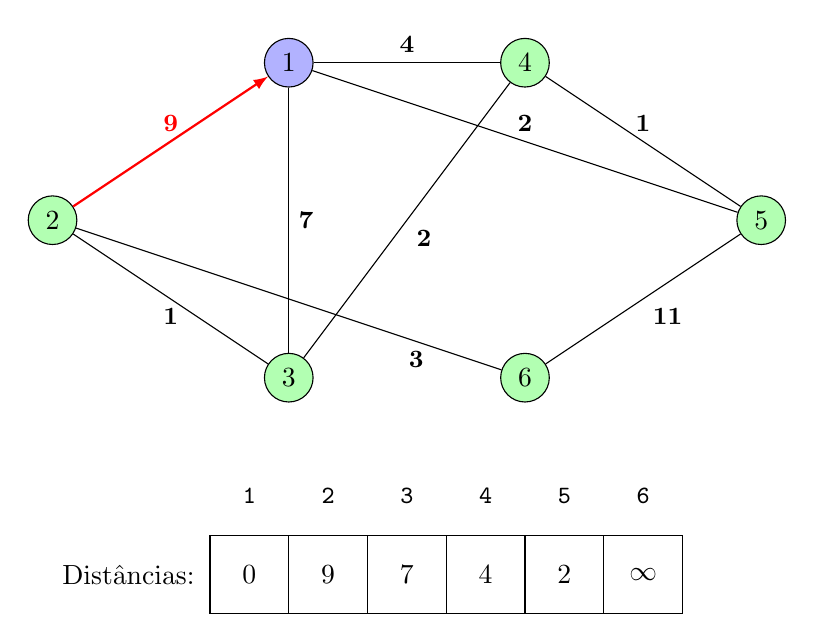
\begin{tikzpicture}
        \node[anchor=west] at (0, 0.5) { Distâncias: };

        \node[circle, draw, fill=blue!30] (a) at (3, 7) {1};
        \node[circle, draw, fill=green!30] (b) at (0, 5) {2};
        \node[circle, draw, fill=green!30] (c) at (3, 3) {3};
        \node[circle, draw, fill=green!30] (d) at (6, 7) {4};
        \node[circle, draw, fill=green!30] (e) at (9, 5) {5};
        \node[circle, draw, fill=green!30] (f) at (6, 3) {6};

        \draw (2, 0) grid (8, 1);

        \node at (2.5, 0.5) { $0$ };
        \node at (3.5, 0.5) { \textcolor{black}{$9$} };
        \node at (4.5, 0.5) { \textcolor{black}{$7$} };
        \node at (5.5, 0.5) { \textcolor{black}{$4$} };
        \node at (6.5, 0.5) { \textcolor{black}{$2$} };
        \node at (7.5, 0.5) { $\infty$ };

        \node at (2.5, 1.5) { \small \texttt{1} };
        \node at (3.5, 1.5) { \small \texttt{2} };
        \node at (4.5, 1.5) { \small \texttt{3} };
        \node at (5.5, 1.5) { \small \texttt{4} };
        \node at (6.5, 1.5) { \small \texttt{5} };
        \node at (7.5, 1.5) { \small \texttt{6} };

        \draw[latex-,thick,red] (a) to node[midway,anchor=south] { \small \bfseries 9 } (b);
        \draw (a) to node[midway,anchor=west] { \small \bfseries 7 } (c);
        \draw (a) to node[midway,anchor=south] { \small \bfseries 4 } (d);
        \draw (a) to node[midway,anchor=south] { \small \bfseries 2 } (e);
        \draw (b) to node[midway,anchor=north] { \small \bfseries 1 } (c);
        \draw (b) to node[pos=0.8,anchor=north] { \small \bfseries 3 } (f);
        \draw (c) to node[midway,anchor=north west] { \small \bfseries 2 } (d);
        \draw (d) to node[midway,anchor=south] { \small \bfseries 1 } (e);
        \draw (e) to node[midway,anchor=north west] { \small \bfseries 11 } (f);

    \end{tikzpicture}

\end{frame}

\begin{frame}[fragile]{Visualização do algoritmo de Bellman-Ford}

    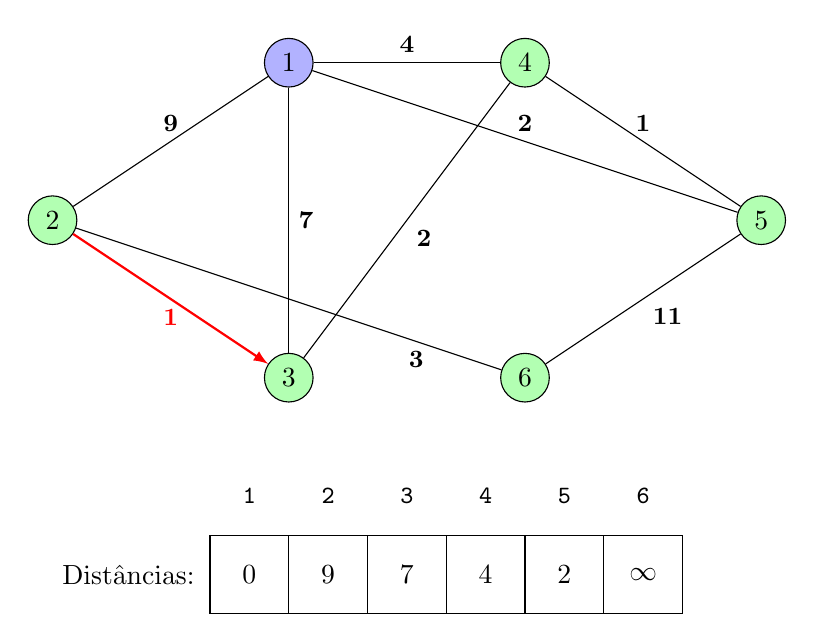
\begin{tikzpicture}
        \node[anchor=west] at (0, 0.5) { Distâncias: };

        \node[circle, draw, fill=blue!30] (a) at (3, 7) {1};
        \node[circle, draw, fill=green!30] (b) at (0, 5) {2};
        \node[circle, draw, fill=green!30] (c) at (3, 3) {3};
        \node[circle, draw, fill=green!30] (d) at (6, 7) {4};
        \node[circle, draw, fill=green!30] (e) at (9, 5) {5};
        \node[circle, draw, fill=green!30] (f) at (6, 3) {6};

        \draw (2, 0) grid (8, 1);

        \node at (2.5, 0.5) { $0$ };
        \node at (3.5, 0.5) { \textcolor{black}{$9$} };
        \node at (4.5, 0.5) { \textcolor{black}{$7$} };
        \node at (5.5, 0.5) { \textcolor{black}{$4$} };
        \node at (6.5, 0.5) { \textcolor{black}{$2$} };
        \node at (7.5, 0.5) { $\infty$ };

        \node at (2.5, 1.5) { \small \texttt{1} };
        \node at (3.5, 1.5) { \small \texttt{2} };
        \node at (4.5, 1.5) { \small \texttt{3} };
        \node at (5.5, 1.5) { \small \texttt{4} };
        \node at (6.5, 1.5) { \small \texttt{5} };
        \node at (7.5, 1.5) { \small \texttt{6} };

        \draw (a) to node[midway,anchor=south] { \small \bfseries 9 } (b);
        \draw (a) to node[midway,anchor=west] { \small \bfseries 7 } (c);
        \draw (a) to node[midway,anchor=south] { \small \bfseries 4 } (d);
        \draw (a) to node[midway,anchor=south] { \small \bfseries 2 } (e);
        %\draw (b) to node[midway,anchor=north] { \small \bfseries 1 } (c);
        \draw[-latex,thick,red] (b) to node[midway,anchor=north] { \small \bfseries 1 } (c);
        \draw (b) to node[pos=0.8,anchor=north] { \small \bfseries 3 } (f);
        \draw (c) to node[midway,anchor=north west] { \small \bfseries 2 } (d);
        \draw (d) to node[midway,anchor=south] { \small \bfseries 1 } (e);
        \draw (e) to node[midway,anchor=north west] { \small \bfseries 11 } (f);

    \end{tikzpicture}

\end{frame}

\begin{frame}[fragile]{Visualização do algoritmo de Bellman-Ford}

    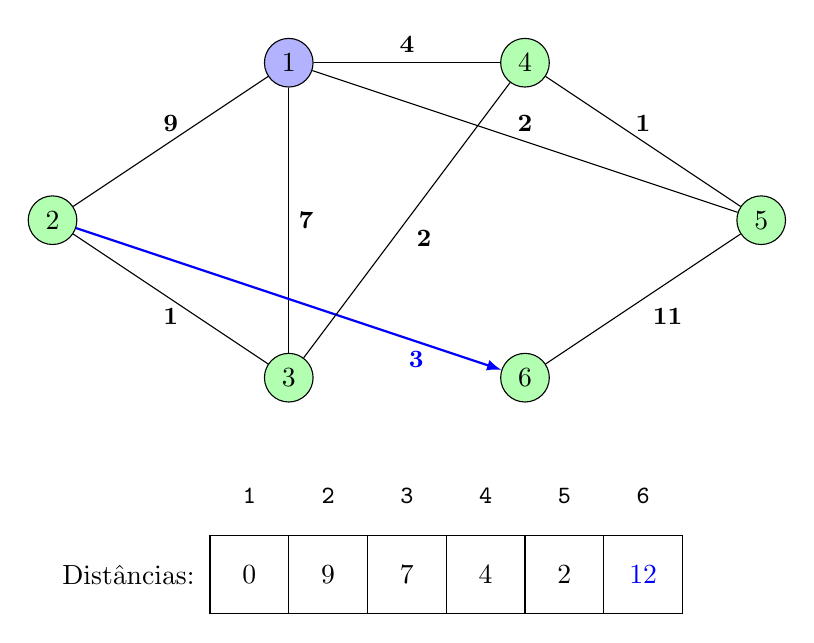
\begin{tikzpicture}
        \node[anchor=west] at (0, 0.5) { Distâncias: };

        \node[circle, draw, fill=blue!30] (a) at (3, 7) {1};
        \node[circle, draw, fill=green!30] (b) at (0, 5) {2};
        \node[circle, draw, fill=green!30] (c) at (3, 3) {3};
        \node[circle, draw, fill=green!30] (d) at (6, 7) {4};
        \node[circle, draw, fill=green!30] (e) at (9, 5) {5};
        \node[circle, draw, fill=green!30] (f) at (6, 3) {6};

        \draw (2, 0) grid (8, 1);

        \node at (2.5, 0.5) { $0$ };
        \node at (3.5, 0.5) { \textcolor{black}{$9$} };
        \node at (4.5, 0.5) { \textcolor{black}{$7$} };
        \node at (5.5, 0.5) { \textcolor{black}{$4$} };
        \node at (6.5, 0.5) { \textcolor{black}{$2$} };
        \node at (7.5, 0.5) { \textcolor{blue}{$12$} };

        \node at (2.5, 1.5) { \small \texttt{1} };
        \node at (3.5, 1.5) { \small \texttt{2} };
        \node at (4.5, 1.5) { \small \texttt{3} };
        \node at (5.5, 1.5) { \small \texttt{4} };
        \node at (6.5, 1.5) { \small \texttt{5} };
        \node at (7.5, 1.5) { \small \texttt{6} };

        \draw (a) to node[midway,anchor=south] { \small \bfseries 9 } (b);
        \draw (a) to node[midway,anchor=west] { \small \bfseries 7 } (c);
        \draw (a) to node[midway,anchor=south] { \small \bfseries 4 } (d);
        \draw (a) to node[midway,anchor=south] { \small \bfseries 2 } (e);
        \draw (b) to node[midway,anchor=north] { \small \bfseries 1 } (c);
        %\draw (b) to node[pos=0.8,anchor=north] { \small \bfseries 3 } (f);
        \draw[-latex,thick,blue] (b) to node[pos=0.8,anchor=north] { \small \bfseries 3 } (f);
        \draw (c) to node[midway,anchor=north west] { \small \bfseries 2 } (d);
        \draw (d) to node[midway,anchor=south] { \small \bfseries 1 } (e);
        \draw (e) to node[midway,anchor=north west] { \small \bfseries 11 } (f);

    \end{tikzpicture}

\end{frame}

\begin{frame}[fragile]{Visualização do algoritmo de Bellman-Ford}

    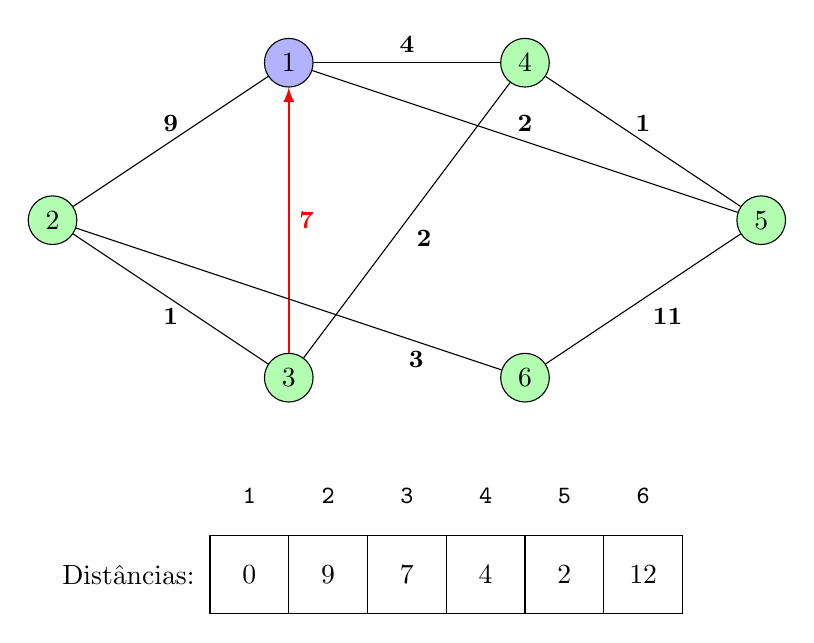
\begin{tikzpicture}
        \node[anchor=west] at (0, 0.5) { Distâncias: };

        \node[circle, draw, fill=blue!30] (a) at (3, 7) {1};
        \node[circle, draw, fill=green!30] (b) at (0, 5) {2};
        \node[circle, draw, fill=green!30] (c) at (3, 3) {3};
        \node[circle, draw, fill=green!30] (d) at (6, 7) {4};
        \node[circle, draw, fill=green!30] (e) at (9, 5) {5};
        \node[circle, draw, fill=green!30] (f) at (6, 3) {6};

        \draw (2, 0) grid (8, 1);

        \node at (2.5, 0.5) { $0$ };
        \node at (3.5, 0.5) { \textcolor{black}{$9$} };
        \node at (4.5, 0.5) { \textcolor{black}{$7$} };
        \node at (5.5, 0.5) { \textcolor{black}{$4$} };
        \node at (6.5, 0.5) { \textcolor{black}{$2$} };
        \node at (7.5, 0.5) { \textcolor{black}{$12$} };

        \node at (2.5, 1.5) { \small \texttt{1} };
        \node at (3.5, 1.5) { \small \texttt{2} };
        \node at (4.5, 1.5) { \small \texttt{3} };
        \node at (5.5, 1.5) { \small \texttt{4} };
        \node at (6.5, 1.5) { \small \texttt{5} };
        \node at (7.5, 1.5) { \small \texttt{6} };

        \draw (a) to node[midway,anchor=south] { \small \bfseries 9 } (b);
        %\draw (a) to node[midway,anchor=west] { \small \bfseries 7 } (c);
        \draw[latex-,thick,red] (a) to node[midway,anchor=west] { \small \bfseries 7 } (c);
        \draw (a) to node[midway,anchor=south] { \small \bfseries 4 } (d);
        \draw (a) to node[midway,anchor=south] { \small \bfseries 2 } (e);
        \draw (b) to node[midway,anchor=north] { \small \bfseries 1 } (c);
        \draw (b) to node[pos=0.8,anchor=north] { \small \bfseries 3 } (f);
        \draw (c) to node[midway,anchor=north west] { \small \bfseries 2 } (d);
        \draw (d) to node[midway,anchor=south] { \small \bfseries 1 } (e);
        \draw (e) to node[midway,anchor=north west] { \small \bfseries 11 } (f);

    \end{tikzpicture}

\end{frame}

\begin{frame}[fragile]{Visualização do algoritmo de Bellman-Ford}

    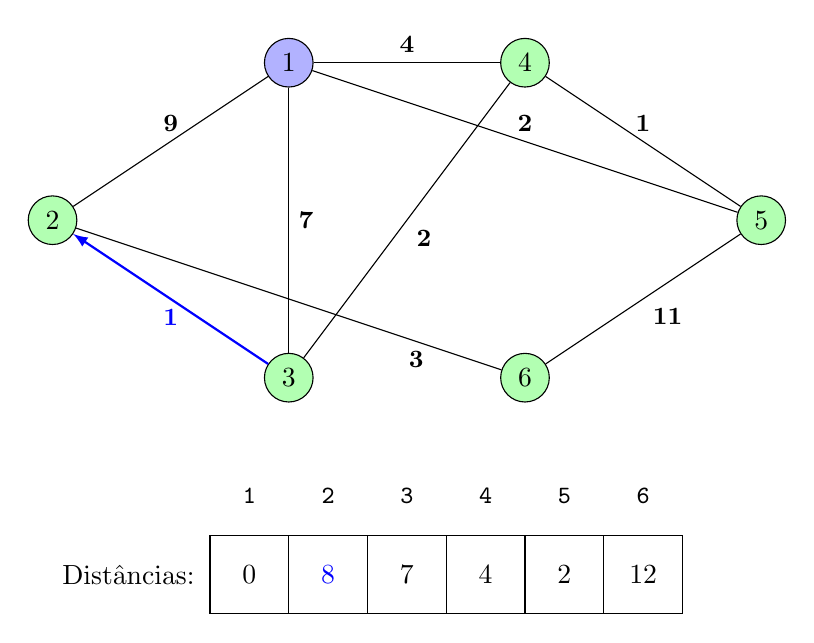
\begin{tikzpicture}
        \node[anchor=west] at (0, 0.5) { Distâncias: };

        \node[circle, draw, fill=blue!30] (a) at (3, 7) {1};
        \node[circle, draw, fill=green!30] (b) at (0, 5) {2};
        \node[circle, draw, fill=green!30] (c) at (3, 3) {3};
        \node[circle, draw, fill=green!30] (d) at (6, 7) {4};
        \node[circle, draw, fill=green!30] (e) at (9, 5) {5};
        \node[circle, draw, fill=green!30] (f) at (6, 3) {6};

        \draw (2, 0) grid (8, 1);

        \node at (2.5, 0.5) { $0$ };
        \node at (3.5, 0.5) { \textcolor{blue}{$8$} };
        \node at (4.5, 0.5) { \textcolor{black}{$7$} };
        \node at (5.5, 0.5) { \textcolor{black}{$4$} };
        \node at (6.5, 0.5) { \textcolor{black}{$2$} };
        \node at (7.5, 0.5) { \textcolor{black}{$12$} };

        \node at (2.5, 1.5) { \small \texttt{1} };
        \node at (3.5, 1.5) { \small \texttt{2} };
        \node at (4.5, 1.5) { \small \texttt{3} };
        \node at (5.5, 1.5) { \small \texttt{4} };
        \node at (6.5, 1.5) { \small \texttt{5} };
        \node at (7.5, 1.5) { \small \texttt{6} };

        \draw (a) to node[midway,anchor=south] { \small \bfseries 9 } (b);
        \draw (a) to node[midway,anchor=west] { \small \bfseries 7 } (c);
        \draw (a) to node[midway,anchor=south] { \small \bfseries 4 } (d);
        \draw (a) to node[midway,anchor=south] { \small \bfseries 2 } (e);
        %\draw (b) to node[midway,anchor=north] { \small \bfseries 1 } (c);
        \draw[latex-,thick,blue] (b) to node[midway,anchor=north] { \small \bfseries 1 } (c);
        \draw (b) to node[pos=0.8,anchor=north] { \small \bfseries 3 } (f);
        \draw (c) to node[midway,anchor=north west] { \small \bfseries 2 } (d);
        \draw (d) to node[midway,anchor=south] { \small \bfseries 1 } (e);
        \draw (e) to node[midway,anchor=north west] { \small \bfseries 11 } (f);

    \end{tikzpicture}

\end{frame}

\begin{frame}[fragile]{Visualização do algoritmo de Bellman-Ford}

    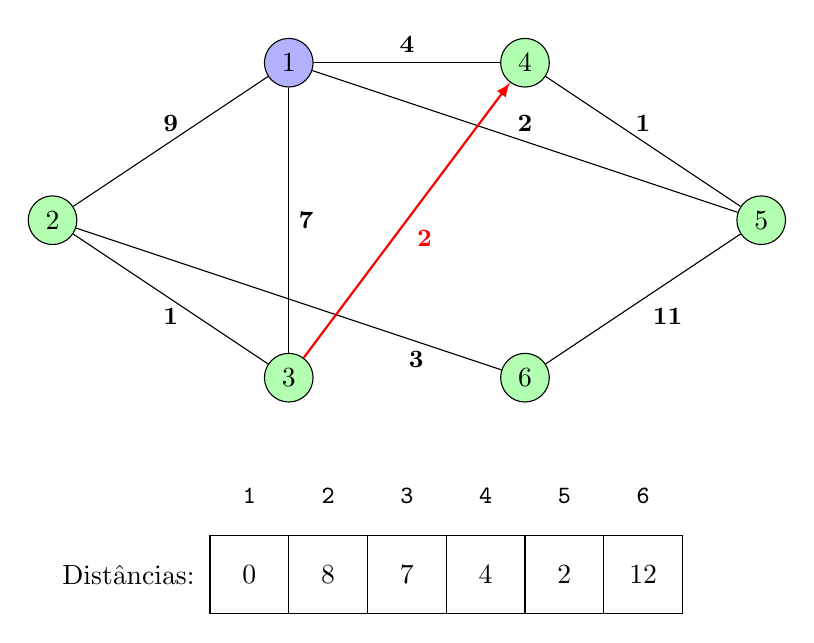
\begin{tikzpicture}
        \node[anchor=west] at (0, 0.5) { Distâncias: };

        \node[circle, draw, fill=blue!30] (a) at (3, 7) {1};
        \node[circle, draw, fill=green!30] (b) at (0, 5) {2};
        \node[circle, draw, fill=green!30] (c) at (3, 3) {3};
        \node[circle, draw, fill=green!30] (d) at (6, 7) {4};
        \node[circle, draw, fill=green!30] (e) at (9, 5) {5};
        \node[circle, draw, fill=green!30] (f) at (6, 3) {6};

        \draw (2, 0) grid (8, 1);

        \node at (2.5, 0.5) { $0$ };
        \node at (3.5, 0.5) { \textcolor{black}{$8$} };
        \node at (4.5, 0.5) { \textcolor{black}{$7$} };
        \node at (5.5, 0.5) { \textcolor{black}{$4$} };
        \node at (6.5, 0.5) { \textcolor{black}{$2$} };
        \node at (7.5, 0.5) { \textcolor{black}{$12$} };

        \node at (2.5, 1.5) { \small \texttt{1} };
        \node at (3.5, 1.5) { \small \texttt{2} };
        \node at (4.5, 1.5) { \small \texttt{3} };
        \node at (5.5, 1.5) { \small \texttt{4} };
        \node at (6.5, 1.5) { \small \texttt{5} };
        \node at (7.5, 1.5) { \small \texttt{6} };

        \draw (a) to node[midway,anchor=south] { \small \bfseries 9 } (b);
        \draw (a) to node[midway,anchor=west] { \small \bfseries 7 } (c);
        \draw (a) to node[midway,anchor=south] { \small \bfseries 4 } (d);
        \draw (a) to node[midway,anchor=south] { \small \bfseries 2 } (e);
        \draw (b) to node[midway,anchor=north] { \small \bfseries 1 } (c);
        \draw (b) to node[pos=0.8,anchor=north] { \small \bfseries 3 } (f);
        %\draw (c) to node[midway,anchor=north west] { \small \bfseries 2 } (d);
        \draw[-latex,thick,red] (c) to node[midway,anchor=north west] { \small \bfseries 2 } (d);
        \draw (d) to node[midway,anchor=south] { \small \bfseries 1 } (e);
        \draw (e) to node[midway,anchor=north west] { \small \bfseries 11 } (f);

    \end{tikzpicture}

\end{frame}

\begin{frame}[fragile]{Visualização do algoritmo de Bellman-Ford}

    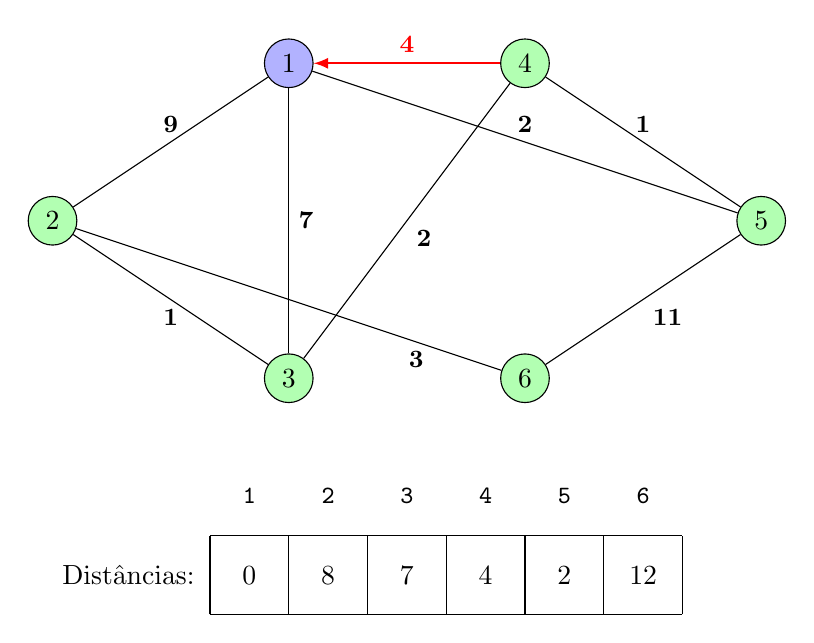
\begin{tikzpicture}
        \node[anchor=west] at (0, 0.5) { Distâncias: };

        \node[circle, draw, fill=blue!30] (a) at (3, 7) {1};
        \node[circle, draw, fill=green!30] (b) at (0, 5) {2};
        \node[circle, draw, fill=green!30] (c) at (3, 3) {3};
        \node[circle, draw, fill=green!30] (d) at (6, 7) {4};
        \node[circle, draw, fill=green!30] (e) at (9, 5) {5};
        \node[circle, draw, fill=green!30] (f) at (6, 3) {6};

        \draw (2, 0) grid (8, 1);

        \node at (2.5, 0.5) { $0$ };
        \node at (3.5, 0.5) { \textcolor{black}{$8$} };
        \node at (4.5, 0.5) { \textcolor{black}{$7$} };
        \node at (5.5, 0.5) { \textcolor{black}{$4$} };
        \node at (6.5, 0.5) { \textcolor{black}{$2$} };
        \node at (7.5, 0.5) { \textcolor{black}{$12$} };

        \node at (2.5, 1.5) { \small \texttt{1} };
        \node at (3.5, 1.5) { \small \texttt{2} };
        \node at (4.5, 1.5) { \small \texttt{3} };
        \node at (5.5, 1.5) { \small \texttt{4} };
        \node at (6.5, 1.5) { \small \texttt{5} };
        \node at (7.5, 1.5) { \small \texttt{6} };

        \draw (a) to node[midway,anchor=south] { \small \bfseries 9 } (b);
        \draw (a) to node[midway,anchor=west] { \small \bfseries 7 } (c);
        %\draw (a) to node[midway,anchor=south] { \small \bfseries 4 } (d);
        \draw[latex-,thick,red] (a) to node[midway,anchor=south] { \small \bfseries 4 } (d);
        \draw (a) to node[midway,anchor=south] { \small \bfseries 2 } (e);
        \draw (b) to node[midway,anchor=north] { \small \bfseries 1 } (c);
        \draw (b) to node[pos=0.8,anchor=north] { \small \bfseries 3 } (f);
        \draw (c) to node[midway,anchor=north west] { \small \bfseries 2 } (d);
        \draw (d) to node[midway,anchor=south] { \small \bfseries 1 } (e);
        \draw (e) to node[midway,anchor=north west] { \small \bfseries 11 } (f);

    \end{tikzpicture}

\end{frame}

\begin{frame}[fragile]{Visualização do algoritmo de Bellman-Ford}

    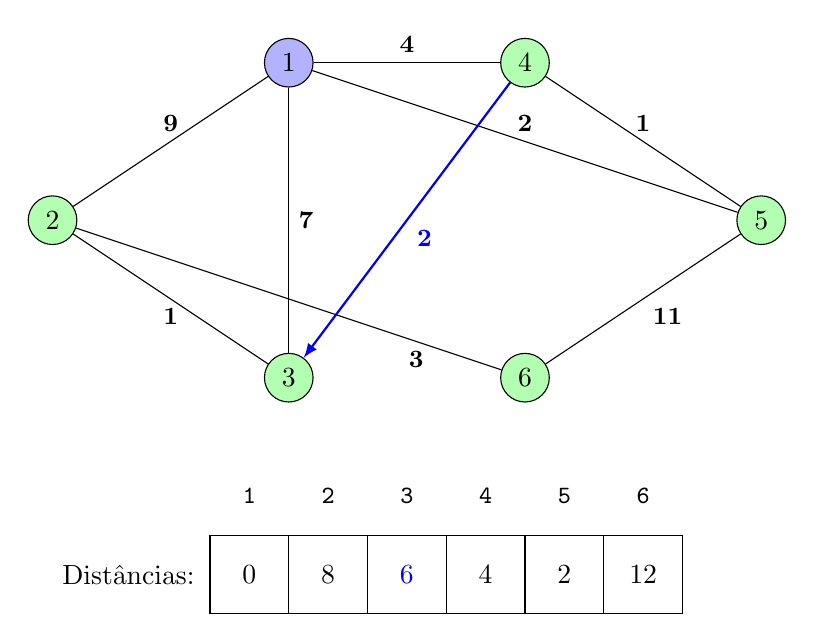
\begin{tikzpicture}
        \node[anchor=west] at (0, 0.5) { Distâncias: };

        \node[circle, draw, fill=blue!30] (a) at (3, 7) {1};
        \node[circle, draw, fill=green!30] (b) at (0, 5) {2};
        \node[circle, draw, fill=green!30] (c) at (3, 3) {3};
        \node[circle, draw, fill=green!30] (d) at (6, 7) {4};
        \node[circle, draw, fill=green!30] (e) at (9, 5) {5};
        \node[circle, draw, fill=green!30] (f) at (6, 3) {6};

        \draw (2, 0) grid (8, 1);

        \node at (2.5, 0.5) { $0$ };
        \node at (3.5, 0.5) { \textcolor{black}{$8$} };
        \node at (4.5, 0.5) { \textcolor{blue}{$6$} };
        \node at (5.5, 0.5) { \textcolor{black}{$4$} };
        \node at (6.5, 0.5) { \textcolor{black}{$2$} };
        \node at (7.5, 0.5) { \textcolor{black}{$12$} };

        \node at (2.5, 1.5) { \small \texttt{1} };
        \node at (3.5, 1.5) { \small \texttt{2} };
        \node at (4.5, 1.5) { \small \texttt{3} };
        \node at (5.5, 1.5) { \small \texttt{4} };
        \node at (6.5, 1.5) { \small \texttt{5} };
        \node at (7.5, 1.5) { \small \texttt{6} };

        \draw (a) to node[midway,anchor=south] { \small \bfseries 9 } (b);
        \draw (a) to node[midway,anchor=west] { \small \bfseries 7 } (c);
        \draw (a) to node[midway,anchor=south] { \small \bfseries 4 } (d);
        \draw (a) to node[midway,anchor=south] { \small \bfseries 2 } (e);
        \draw (b) to node[midway,anchor=north] { \small \bfseries 1 } (c);
        \draw (b) to node[pos=0.8,anchor=north] { \small \bfseries 3 } (f);
        \draw[latex-,thick,blue] (c) to node[midway,anchor=north west] { \small \bfseries 2 } (d);
        \draw (d) to node[midway,anchor=south] { \small \bfseries 1 } (e);
        \draw (e) to node[midway,anchor=north west] { \small \bfseries 11 } (f);

    \end{tikzpicture}

\end{frame}



\begin{frame}[fragile]{Visualização do algoritmo de Bellman-Ford}

    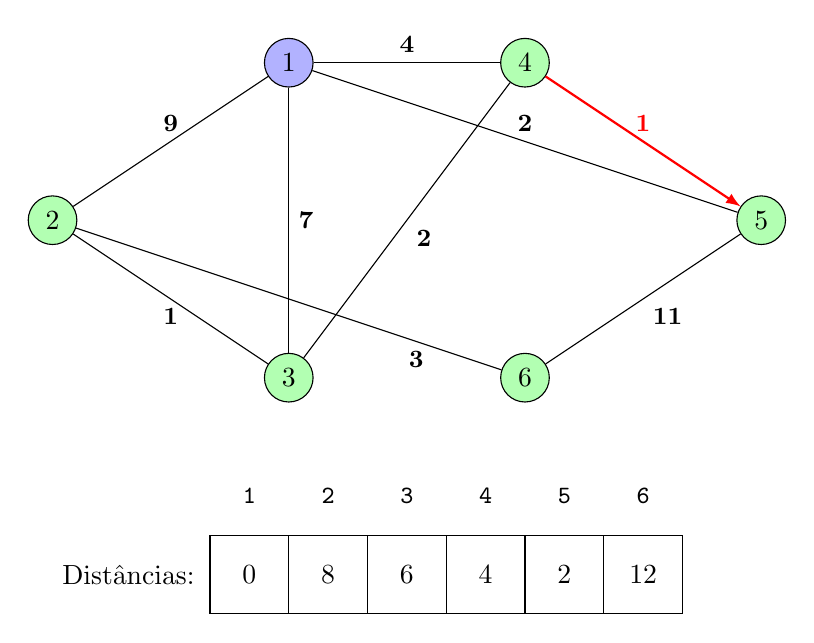
\begin{tikzpicture}
        \node[anchor=west] at (0, 0.5) { Distâncias: };

        \node[circle, draw, fill=blue!30] (a) at (3, 7) {1};
        \node[circle, draw, fill=green!30] (b) at (0, 5) {2};
        \node[circle, draw, fill=green!30] (c) at (3, 3) {3};
        \node[circle, draw, fill=green!30] (d) at (6, 7) {4};
        \node[circle, draw, fill=green!30] (e) at (9, 5) {5};
        \node[circle, draw, fill=green!30] (f) at (6, 3) {6};

        \draw (2, 0) grid (8, 1);

        \node at (2.5, 0.5) { $0$ };
        \node at (3.5, 0.5) { \textcolor{black}{$8$} };
        \node at (4.5, 0.5) { \textcolor{black}{$6$} };
        \node at (5.5, 0.5) { \textcolor{black}{$4$} };
        \node at (6.5, 0.5) { \textcolor{black}{$2$} };
        \node at (7.5, 0.5) { \textcolor{black}{$12$} };

        \node at (2.5, 1.5) { \small \texttt{1} };
        \node at (3.5, 1.5) { \small \texttt{2} };
        \node at (4.5, 1.5) { \small \texttt{3} };
        \node at (5.5, 1.5) { \small \texttt{4} };
        \node at (6.5, 1.5) { \small \texttt{5} };
        \node at (7.5, 1.5) { \small \texttt{6} };

        \draw (a) to node[midway,anchor=south] { \small \bfseries 9 } (b);
        \draw (a) to node[midway,anchor=west] { \small \bfseries 7 } (c);
        \draw (a) to node[midway,anchor=south] { \small \bfseries 4 } (d);
        \draw (a) to node[midway,anchor=south] { \small \bfseries 2 } (e);
        \draw (b) to node[midway,anchor=north] { \small \bfseries 1 } (c);
        \draw (b) to node[pos=0.8,anchor=north] { \small \bfseries 3 } (f);
        \draw (c) to node[midway,anchor=north west] { \small \bfseries 2 } (d);
        %\draw (d) to node[midway,anchor=south] { \small \bfseries 1 } (e);
        \draw[-latex,thick,red] (d) to node[midway,anchor=south] { \small \bfseries 1 } (e);
        \draw (e) to node[midway,anchor=north west] { \small \bfseries 11 } (f);

    \end{tikzpicture}

\end{frame}

\begin{frame}[fragile]{Visualização do algoritmo de Bellman-Ford}

    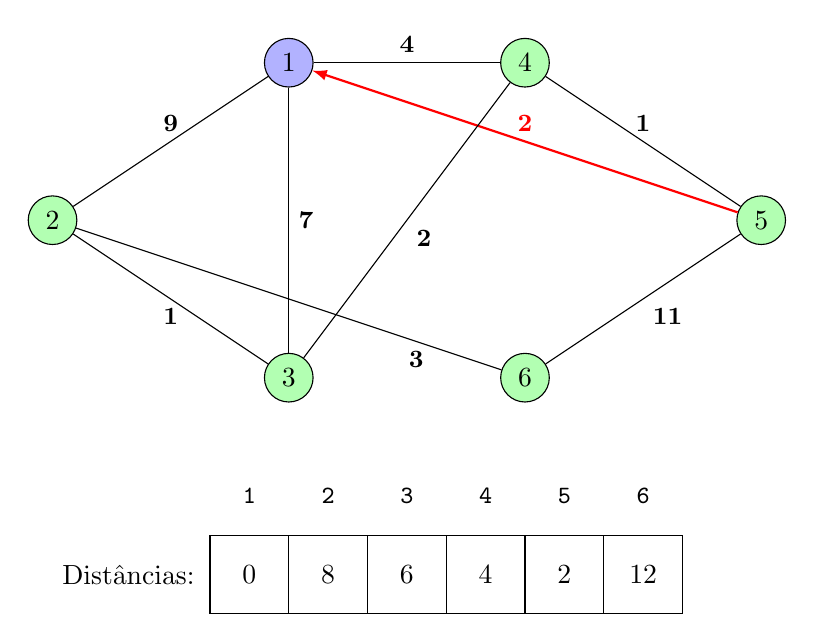
\begin{tikzpicture}
        \node[anchor=west] at (0, 0.5) { Distâncias: };

        \node[circle, draw, fill=blue!30] (a) at (3, 7) {1};
        \node[circle, draw, fill=green!30] (b) at (0, 5) {2};
        \node[circle, draw, fill=green!30] (c) at (3, 3) {3};
        \node[circle, draw, fill=green!30] (d) at (6, 7) {4};
        \node[circle, draw, fill=green!30] (e) at (9, 5) {5};
        \node[circle, draw, fill=green!30] (f) at (6, 3) {6};

        \draw (2, 0) grid (8, 1);

        \node at (2.5, 0.5) { $0$ };
        \node at (3.5, 0.5) { \textcolor{black}{$8$} };
        \node at (4.5, 0.5) { \textcolor{black}{$6$} };
        \node at (5.5, 0.5) { \textcolor{black}{$4$} };
        \node at (6.5, 0.5) { \textcolor{black}{$2$} };
        \node at (7.5, 0.5) { \textcolor{black}{$12$} };

        \node at (2.5, 1.5) { \small \texttt{1} };
        \node at (3.5, 1.5) { \small \texttt{2} };
        \node at (4.5, 1.5) { \small \texttt{3} };
        \node at (5.5, 1.5) { \small \texttt{4} };
        \node at (6.5, 1.5) { \small \texttt{5} };
        \node at (7.5, 1.5) { \small \texttt{6} };

        \draw (a) to node[midway,anchor=south] { \small \bfseries 9 } (b);
        \draw (a) to node[midway,anchor=west] { \small \bfseries 7 } (c);
        \draw (a) to node[midway,anchor=south] { \small \bfseries 4 } (d);
        %\draw (a) to node[midway,anchor=south] { \small \bfseries 2 } (e);
        \draw[latex-,thick,red] (a) to node[midway,anchor=south] { \small \bfseries 2 } (e);
        \draw (b) to node[midway,anchor=north] { \small \bfseries 1 } (c);
        \draw (b) to node[pos=0.8,anchor=north] { \small \bfseries 3 } (f);
        \draw (c) to node[midway,anchor=north west] { \small \bfseries 2 } (d);
        \draw (d) to node[midway,anchor=south] { \small \bfseries 1 } (e);
        \draw (e) to node[midway,anchor=north west] { \small \bfseries 11 } (f);

    \end{tikzpicture}

\end{frame}

\begin{frame}[fragile]{Visualização do algoritmo de Bellman-Ford}

    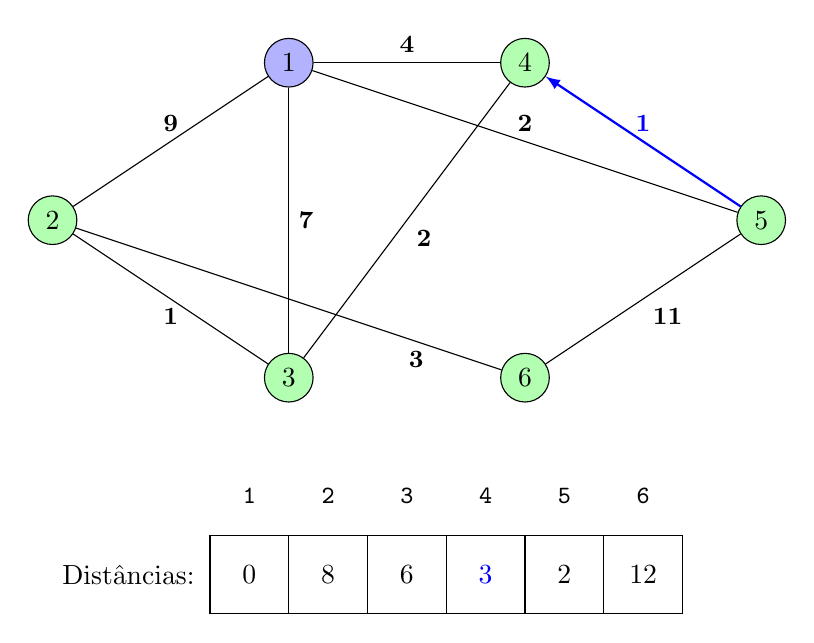
\begin{tikzpicture}
        \node[anchor=west] at (0, 0.5) { Distâncias: };

        \node[circle, draw, fill=blue!30] (a) at (3, 7) {1};
        \node[circle, draw, fill=green!30] (b) at (0, 5) {2};
        \node[circle, draw, fill=green!30] (c) at (3, 3) {3};
        \node[circle, draw, fill=green!30] (d) at (6, 7) {4};
        \node[circle, draw, fill=green!30] (e) at (9, 5) {5};
        \node[circle, draw, fill=green!30] (f) at (6, 3) {6};

        \draw (2, 0) grid (8, 1);

        \node at (2.5, 0.5) { $0$ };
        \node at (3.5, 0.5) { \textcolor{black}{$8$} };
        \node at (4.5, 0.5) { \textcolor{black}{$6$} };
        \node at (5.5, 0.5) { \textcolor{blue}{$3$} };
        \node at (6.5, 0.5) { \textcolor{black}{$2$} };
        \node at (7.5, 0.5) { \textcolor{black}{$12$} };

        \node at (2.5, 1.5) { \small \texttt{1} };
        \node at (3.5, 1.5) { \small \texttt{2} };
        \node at (4.5, 1.5) { \small \texttt{3} };
        \node at (5.5, 1.5) { \small \texttt{4} };
        \node at (6.5, 1.5) { \small \texttt{5} };
        \node at (7.5, 1.5) { \small \texttt{6} };

        \draw (a) to node[midway,anchor=south] { \small \bfseries 9 } (b);
        \draw (a) to node[midway,anchor=west] { \small \bfseries 7 } (c);
        \draw (a) to node[midway,anchor=south] { \small \bfseries 4 } (d);
        \draw (a) to node[midway,anchor=south] { \small \bfseries 2 } (e);
        \draw (b) to node[midway,anchor=north] { \small \bfseries 1 } (c);
        \draw (b) to node[pos=0.8,anchor=north] { \small \bfseries 3 } (f);
        \draw (c) to node[midway,anchor=north west] { \small \bfseries 2 } (d);
        %\draw (d) to node[midway,anchor=south] { \small \bfseries 1 } (e);
        \draw[latex-,thick,blue] (d) to node[midway,anchor=south] { \small \bfseries 1 } (e);
        \draw (e) to node[midway,anchor=north west] { \small \bfseries 11 } (f);

    \end{tikzpicture}

\end{frame}

\begin{frame}[fragile]{Visualização do algoritmo de Bellman-Ford}

    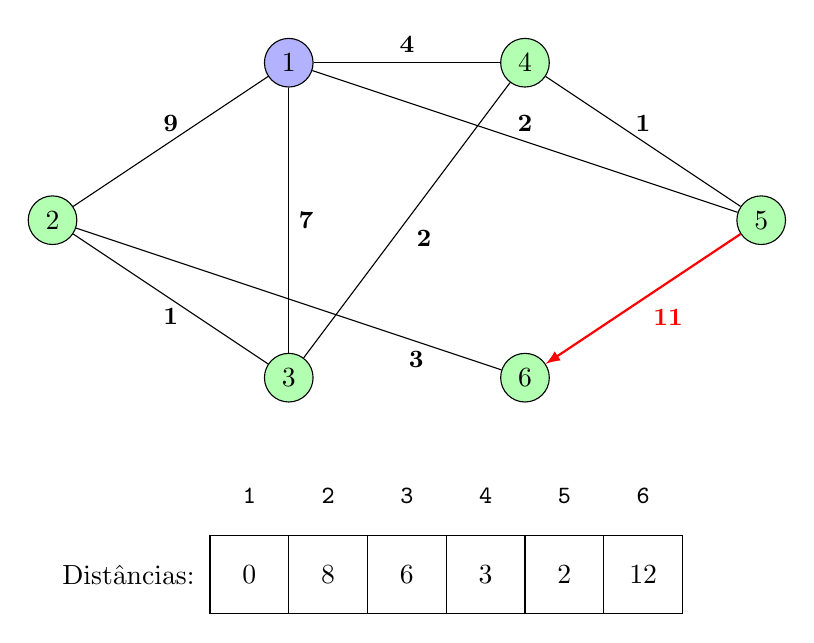
\begin{tikzpicture}
        \node[anchor=west] at (0, 0.5) { Distâncias: };

        \node[circle, draw, fill=blue!30] (a) at (3, 7) {1};
        \node[circle, draw, fill=green!30] (b) at (0, 5) {2};
        \node[circle, draw, fill=green!30] (c) at (3, 3) {3};
        \node[circle, draw, fill=green!30] (d) at (6, 7) {4};
        \node[circle, draw, fill=green!30] (e) at (9, 5) {5};
        \node[circle, draw, fill=green!30] (f) at (6, 3) {6};

        \draw (2, 0) grid (8, 1);

        \node at (2.5, 0.5) { $0$ };
        \node at (3.5, 0.5) { \textcolor{black}{$8$} };
        \node at (4.5, 0.5) { \textcolor{black}{$6$} };
        \node at (5.5, 0.5) { \textcolor{black}{$3$} };
        \node at (6.5, 0.5) { \textcolor{black}{$2$} };
        \node at (7.5, 0.5) { \textcolor{black}{$12$} };

        \node at (2.5, 1.5) { \small \texttt{1} };
        \node at (3.5, 1.5) { \small \texttt{2} };
        \node at (4.5, 1.5) { \small \texttt{3} };
        \node at (5.5, 1.5) { \small \texttt{4} };
        \node at (6.5, 1.5) { \small \texttt{5} };
        \node at (7.5, 1.5) { \small \texttt{6} };

        \draw (a) to node[midway,anchor=south] { \small \bfseries 9 } (b);
        \draw (a) to node[midway,anchor=west] { \small \bfseries 7 } (c);
        \draw (a) to node[midway,anchor=south] { \small \bfseries 4 } (d);
        \draw (a) to node[midway,anchor=south] { \small \bfseries 2 } (e);
        \draw (b) to node[midway,anchor=north] { \small \bfseries 1 } (c);
        \draw (b) to node[pos=0.8,anchor=north] { \small \bfseries 3 } (f);
        \draw (c) to node[midway,anchor=north west] { \small \bfseries 2 } (d);
        \draw (d) to node[midway,anchor=south] { \small \bfseries 1 } (e);
        %\draw (e) to node[midway,anchor=north west] { \small \bfseries 11 } (f);
        \draw[-latex,thick,red] (e) to node[midway,anchor=north west] { \small \bfseries 11 } (f);

    \end{tikzpicture}

\end{frame}


\begin{frame}[fragile]{Visualização do algoritmo de Bellman-Ford}

    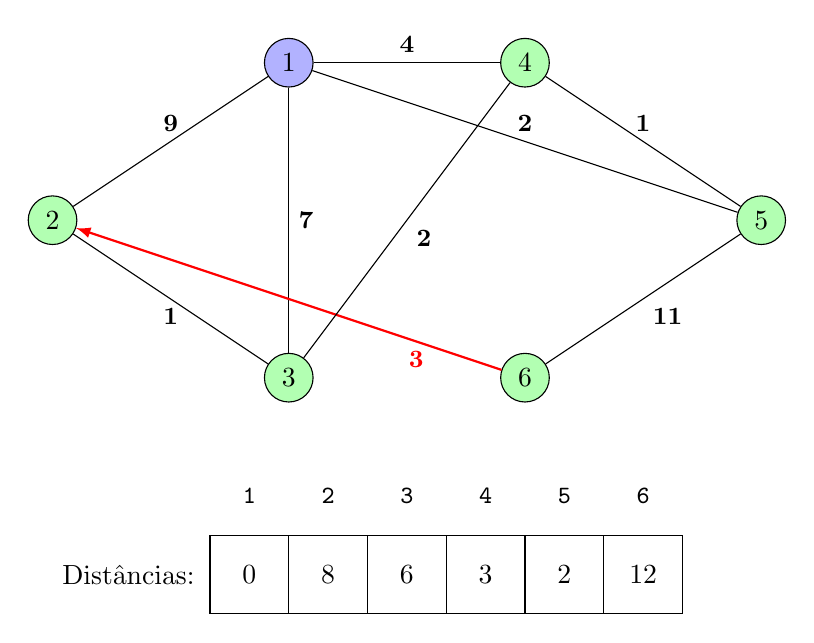
\begin{tikzpicture}
        \node[anchor=west] at (0, 0.5) { Distâncias: };

        \node[circle, draw, fill=blue!30] (a) at (3, 7) {1};
        \node[circle, draw, fill=green!30] (b) at (0, 5) {2};
        \node[circle, draw, fill=green!30] (c) at (3, 3) {3};
        \node[circle, draw, fill=green!30] (d) at (6, 7) {4};
        \node[circle, draw, fill=green!30] (e) at (9, 5) {5};
        \node[circle, draw, fill=green!30] (f) at (6, 3) {6};

        \draw (2, 0) grid (8, 1);

        \node at (2.5, 0.5) { $0$ };
        \node at (3.5, 0.5) { \textcolor{black}{$8$} };
        \node at (4.5, 0.5) { \textcolor{black}{$6$} };
        \node at (5.5, 0.5) { \textcolor{black}{$3$} };
        \node at (6.5, 0.5) { \textcolor{black}{$2$} };
        \node at (7.5, 0.5) { \textcolor{black}{$12$} };

        \node at (2.5, 1.5) { \small \texttt{1} };
        \node at (3.5, 1.5) { \small \texttt{2} };
        \node at (4.5, 1.5) { \small \texttt{3} };
        \node at (5.5, 1.5) { \small \texttt{4} };
        \node at (6.5, 1.5) { \small \texttt{5} };
        \node at (7.5, 1.5) { \small \texttt{6} };

        \draw (a) to node[midway,anchor=south] { \small \bfseries 9 } (b);
        \draw (a) to node[midway,anchor=west] { \small \bfseries 7 } (c);
        \draw (a) to node[midway,anchor=south] { \small \bfseries 4 } (d);
        \draw (a) to node[midway,anchor=south] { \small \bfseries 2 } (e);
        \draw (b) to node[midway,anchor=north] { \small \bfseries 1 } (c);
        %\draw (b) to node[pos=0.8,anchor=north] { \small \bfseries 3 } (f);
        \draw[latex-,thick,red] (b) to node[pos=0.8,anchor=north] { \small \bfseries 3 } (f);
        \draw (c) to node[midway,anchor=north west] { \small \bfseries 2 } (d);
        \draw (d) to node[midway,anchor=south] { \small \bfseries 1 } (e);
        \draw (e) to node[midway,anchor=north west] { \small \bfseries 11 } (f);

    \end{tikzpicture}

\end{frame}

\begin{frame}[fragile]{Visualização do algoritmo de Bellman-Ford}

    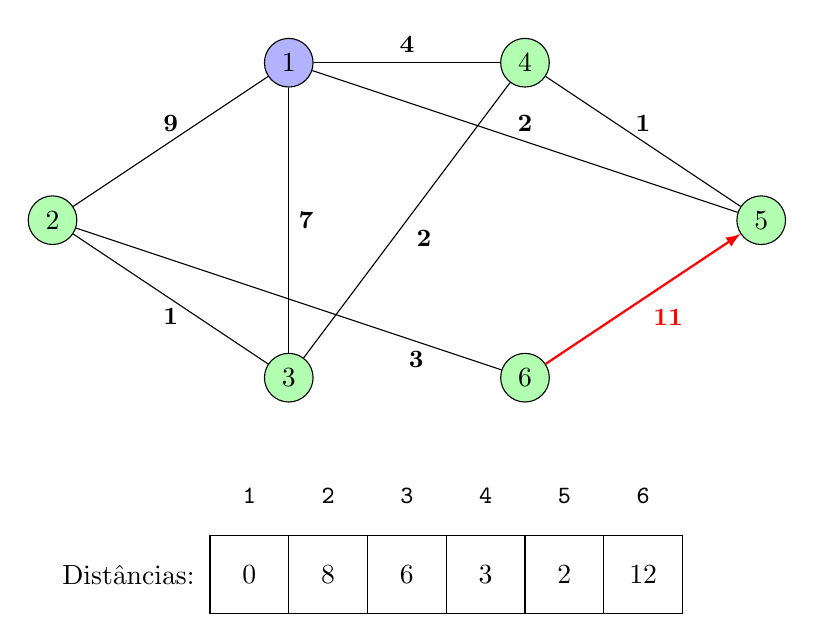
\begin{tikzpicture}
        \node[anchor=west] at (0, 0.5) { Distâncias: };

        \node[circle, draw, fill=blue!30] (a) at (3, 7) {1};
        \node[circle, draw, fill=green!30] (b) at (0, 5) {2};
        \node[circle, draw, fill=green!30] (c) at (3, 3) {3};
        \node[circle, draw, fill=green!30] (d) at (6, 7) {4};
        \node[circle, draw, fill=green!30] (e) at (9, 5) {5};
        \node[circle, draw, fill=green!30] (f) at (6, 3) {6};

        \draw (2, 0) grid (8, 1);

        \node at (2.5, 0.5) { $0$ };
        \node at (3.5, 0.5) { \textcolor{black}{$8$} };
        \node at (4.5, 0.5) { \textcolor{black}{$6$} };
        \node at (5.5, 0.5) { \textcolor{black}{$3$} };
        \node at (6.5, 0.5) { \textcolor{black}{$2$} };
        \node at (7.5, 0.5) { \textcolor{black}{$12$} };

        \node at (2.5, 1.5) { \small \texttt{1} };
        \node at (3.5, 1.5) { \small \texttt{2} };
        \node at (4.5, 1.5) { \small \texttt{3} };
        \node at (5.5, 1.5) { \small \texttt{4} };
        \node at (6.5, 1.5) { \small \texttt{5} };
        \node at (7.5, 1.5) { \small \texttt{6} };

        \draw (a) to node[midway,anchor=south] { \small \bfseries 9 } (b);
        \draw (a) to node[midway,anchor=west] { \small \bfseries 7 } (c);
        \draw (a) to node[midway,anchor=south] { \small \bfseries 4 } (d);
        \draw (a) to node[midway,anchor=south] { \small \bfseries 2 } (e);
        \draw (b) to node[midway,anchor=north] { \small \bfseries 1 } (c);
        \draw (b) to node[pos=0.8,anchor=north] { \small \bfseries 3 } (f);
        \draw (c) to node[midway,anchor=north west] { \small \bfseries 2 } (d);
        \draw (d) to node[midway,anchor=south] { \small \bfseries 1 } (e);
        %\draw (e) to node[midway,anchor=north west] { \small \bfseries 11 } (f);
        \draw[latex-,thick,red] (e) to node[midway,anchor=north west] { \small \bfseries 11 } (f);

    \end{tikzpicture}

\end{frame}

\begin{frame}[fragile]{Visualização do algoritmo de Bellman-Ford}

    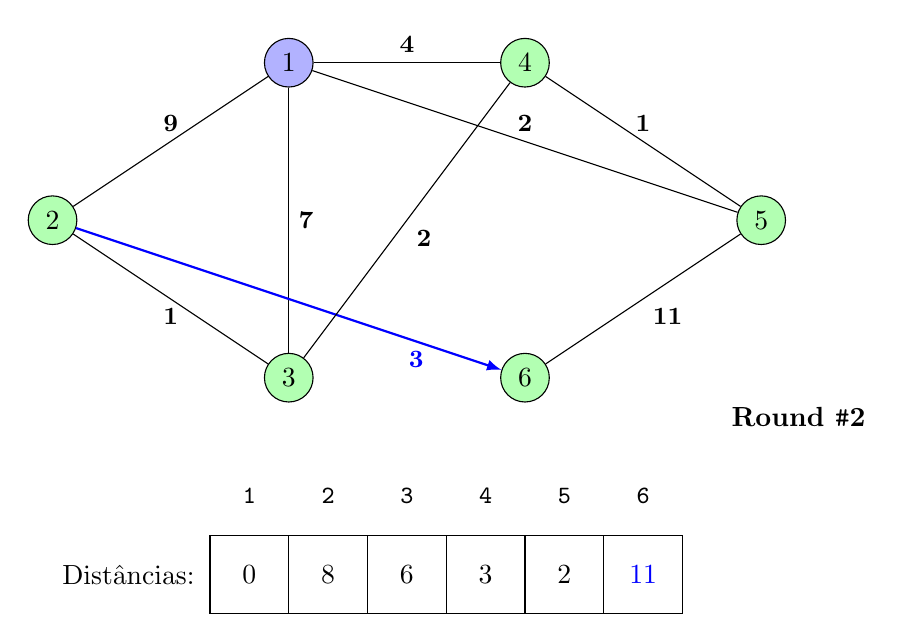
\begin{tikzpicture}
        \node[anchor=west] at (0, 0.5) { Distâncias: };
        \node[anchor=west] at (8.5, 2.5) { \bfseries Round \texttt{\#}2 };

        \node[circle, draw, fill=blue!30] (a) at (3, 7) {1};
        \node[circle, draw, fill=green!30] (b) at (0, 5) {2};
        \node[circle, draw, fill=green!30] (c) at (3, 3) {3};
        \node[circle, draw, fill=green!30] (d) at (6, 7) {4};
        \node[circle, draw, fill=green!30] (e) at (9, 5) {5};
        \node[circle, draw, fill=green!30] (f) at (6, 3) {6};

        \draw (2, 0) grid (8, 1);

        \node at (2.5, 0.5) { $0$ };
        \node at (3.5, 0.5) { \textcolor{black}{$8$} };
        \node at (4.5, 0.5) { \textcolor{black}{$6$} };
        \node at (5.5, 0.5) { \textcolor{black}{$3$} };
        \node at (6.5, 0.5) { \textcolor{black}{$2$} };
        \node at (7.5, 0.5) { \textcolor{blue}{$11$} };

        \node at (2.5, 1.5) { \small \texttt{1} };
        \node at (3.5, 1.5) { \small \texttt{2} };
        \node at (4.5, 1.5) { \small \texttt{3} };
        \node at (5.5, 1.5) { \small \texttt{4} };
        \node at (6.5, 1.5) { \small \texttt{5} };
        \node at (7.5, 1.5) { \small \texttt{6} };

        \draw (a) to node[midway,anchor=south] { \small \bfseries 9 } (b);
        \draw (a) to node[midway,anchor=west] { \small \bfseries 7 } (c);
        \draw (a) to node[midway,anchor=south] { \small \bfseries 4 } (d);
        \draw (a) to node[midway,anchor=south] { \small \bfseries 2 } (e);
        \draw (b) to node[midway,anchor=north] { \small \bfseries 1 } (c);
        \draw[-latex,thick,blue] (b) to node[pos=0.8,anchor=north] { \small \bfseries 3 } (f);
        \draw (c) to node[midway,anchor=north west] { \small \bfseries 2 } (d);
        \draw (d) to node[midway,anchor=south] { \small \bfseries 1 } (e);
        \draw (e) to node[midway,anchor=north west] { \small \bfseries 11 } (f);

    \end{tikzpicture}

\end{frame}

\begin{frame}[fragile]{Visualização do algoritmo de Bellman-Ford}

    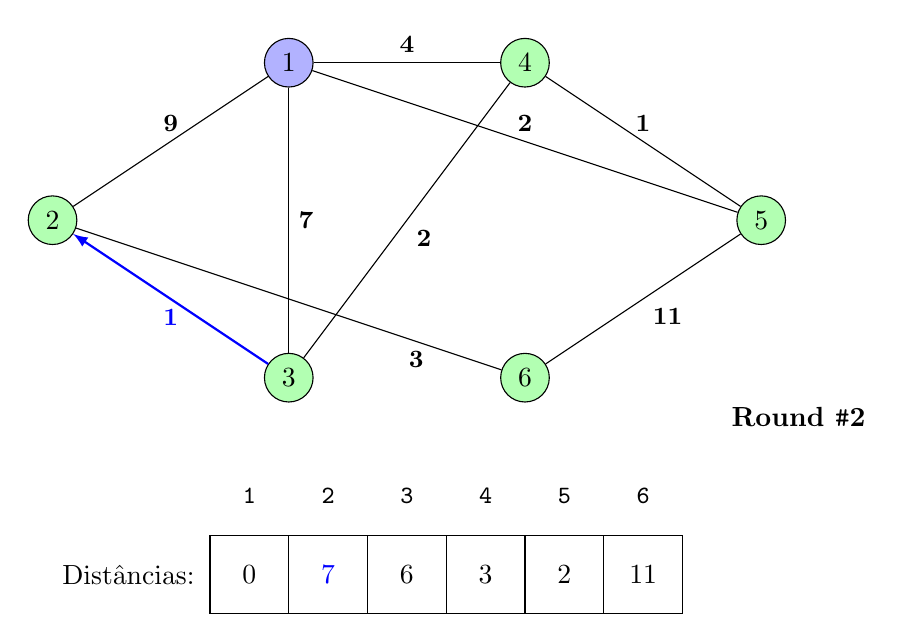
\begin{tikzpicture}
        \node[anchor=west] at (0, 0.5) { Distâncias: };
        \node[anchor=west] at (8.5, 2.5) { \bfseries Round \texttt{\#}2 };

        \node[circle, draw, fill=blue!30] (a) at (3, 7) {1};
        \node[circle, draw, fill=green!30] (b) at (0, 5) {2};
        \node[circle, draw, fill=green!30] (c) at (3, 3) {3};
        \node[circle, draw, fill=green!30] (d) at (6, 7) {4};
        \node[circle, draw, fill=green!30] (e) at (9, 5) {5};
        \node[circle, draw, fill=green!30] (f) at (6, 3) {6};

        \draw (2, 0) grid (8, 1);

        \node at (2.5, 0.5) { $0$ };
        \node at (3.5, 0.5) { \textcolor{blue}{$7$} };
        \node at (4.5, 0.5) { \textcolor{black}{$6$} };
        \node at (5.5, 0.5) { \textcolor{black}{$3$} };
        \node at (6.5, 0.5) { \textcolor{black}{$2$} };
        \node at (7.5, 0.5) { \textcolor{black}{$11$} };

        \node at (2.5, 1.5) { \small \texttt{1} };
        \node at (3.5, 1.5) { \small \texttt{2} };
        \node at (4.5, 1.5) { \small \texttt{3} };
        \node at (5.5, 1.5) { \small \texttt{4} };
        \node at (6.5, 1.5) { \small \texttt{5} };
        \node at (7.5, 1.5) { \small \texttt{6} };

        \draw (a) to node[midway,anchor=south] { \small \bfseries 9 } (b);
        \draw (a) to node[midway,anchor=west] { \small \bfseries 7 } (c);
        \draw (a) to node[midway,anchor=south] { \small \bfseries 4 } (d);
        \draw (a) to node[midway,anchor=south] { \small \bfseries 2 } (e);
        %\draw (b) to node[midway,anchor=north] { \small \bfseries 1 } (c);
        \draw[latex-,thick,blue](b) to node[midway,anchor=north] { \small \bfseries 1 } (c);
        \draw (b) to node[pos=0.8,anchor=north] { \small \bfseries 3 } (f);
        \draw (c) to node[midway,anchor=north west] { \small \bfseries 2 } (d);
        \draw (d) to node[midway,anchor=south] { \small \bfseries 1 } (e);
        \draw (e) to node[midway,anchor=north west] { \small \bfseries 11 } (f);

    \end{tikzpicture}

\end{frame}

\begin{frame}[fragile]{Visualização do algoritmo de Bellman-Ford}

    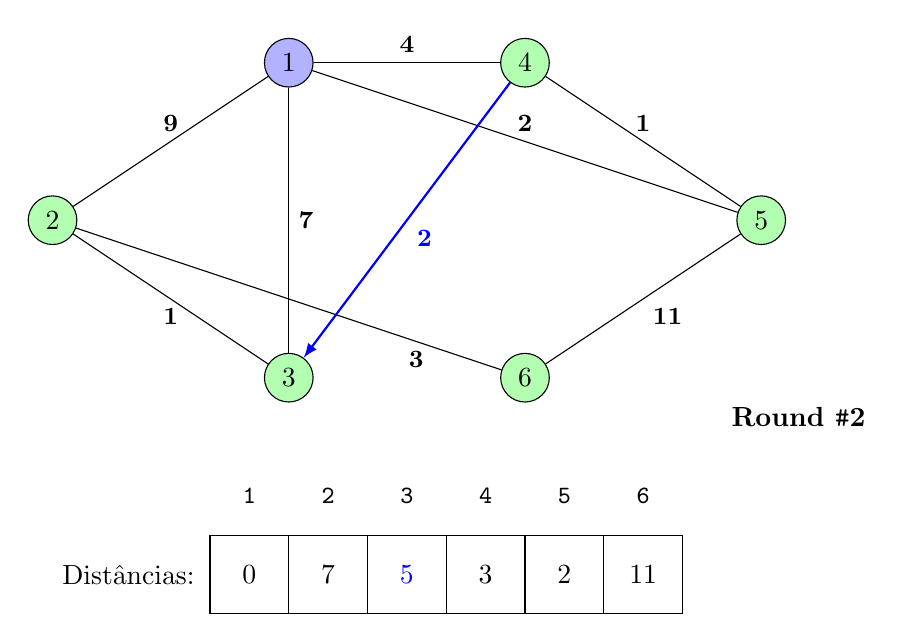
\begin{tikzpicture}
        \node[anchor=west] at (0, 0.5) { Distâncias: };
        \node[anchor=west] at (8.5, 2.5) { \bfseries Round \texttt{\#}2 };

        \node[circle, draw, fill=blue!30] (a) at (3, 7) {1};
        \node[circle, draw, fill=green!30] (b) at (0, 5) {2};
        \node[circle, draw, fill=green!30] (c) at (3, 3) {3};
        \node[circle, draw, fill=green!30] (d) at (6, 7) {4};
        \node[circle, draw, fill=green!30] (e) at (9, 5) {5};
        \node[circle, draw, fill=green!30] (f) at (6, 3) {6};

        \draw (2, 0) grid (8, 1);

        \node at (2.5, 0.5) { $0$ };
        \node at (3.5, 0.5) { \textcolor{black}{$7$} };
        \node at (4.5, 0.5) { \textcolor{blue}{$5$} };
        \node at (5.5, 0.5) { \textcolor{black}{$3$} };
        \node at (6.5, 0.5) { \textcolor{black}{$2$} };
        \node at (7.5, 0.5) { \textcolor{black}{$11$} };

        \node at (2.5, 1.5) { \small \texttt{1} };
        \node at (3.5, 1.5) { \small \texttt{2} };
        \node at (4.5, 1.5) { \small \texttt{3} };
        \node at (5.5, 1.5) { \small \texttt{4} };
        \node at (6.5, 1.5) { \small \texttt{5} };
        \node at (7.5, 1.5) { \small \texttt{6} };

        \draw (a) to node[midway,anchor=south] { \small \bfseries 9 } (b);
        \draw (a) to node[midway,anchor=west] { \small \bfseries 7 } (c);
        \draw (a) to node[midway,anchor=south] { \small \bfseries 4 } (d);
        \draw (a) to node[midway,anchor=south] { \small \bfseries 2 } (e);
        \draw (b) to node[midway,anchor=north] { \small \bfseries 1 } (c);
        \draw (b) to node[pos=0.8,anchor=north] { \small \bfseries 3 } (f);
        %\draw (c) to node[midway,anchor=north west] { \small \bfseries 2 } (d);
        \draw[latex-,thick,blue](c) to node[midway,anchor=north west] { \small \bfseries 2 } (d);
        \draw (d) to node[midway,anchor=south] { \small \bfseries 1 } (e);
        \draw (e) to node[midway,anchor=north west] { \small \bfseries 11 } (f);

    \end{tikzpicture}

\end{frame}

\begin{frame}[fragile]{Visualização do algoritmo de Bellman-Ford}

    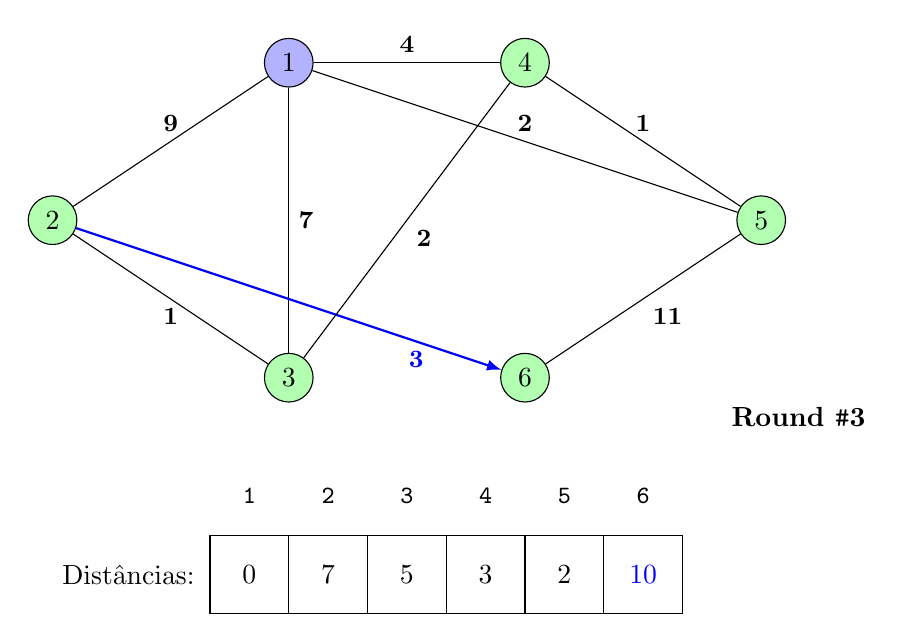
\begin{tikzpicture}
        \node[anchor=west] at (0, 0.5) { Distâncias: };
        \node[anchor=west] at (8.5, 2.5) { \bfseries Round \texttt{\#}3 };

        \node[circle, draw, fill=blue!30] (a) at (3, 7) {1};
        \node[circle, draw, fill=green!30] (b) at (0, 5) {2};
        \node[circle, draw, fill=green!30] (c) at (3, 3) {3};
        \node[circle, draw, fill=green!30] (d) at (6, 7) {4};
        \node[circle, draw, fill=green!30] (e) at (9, 5) {5};
        \node[circle, draw, fill=green!30] (f) at (6, 3) {6};

        \draw (2, 0) grid (8, 1);

        \node at (2.5, 0.5) { $0$ };
        \node at (3.5, 0.5) { \textcolor{black}{$7$} };
        \node at (4.5, 0.5) { \textcolor{black}{$5$} };
        \node at (5.5, 0.5) { \textcolor{black}{$3$} };
        \node at (6.5, 0.5) { \textcolor{black}{$2$} };
        \node at (7.5, 0.5) { \textcolor{blue}{$10$} };

        \node at (2.5, 1.5) { \small \texttt{1} };
        \node at (3.5, 1.5) { \small \texttt{2} };
        \node at (4.5, 1.5) { \small \texttt{3} };
        \node at (5.5, 1.5) { \small \texttt{4} };
        \node at (6.5, 1.5) { \small \texttt{5} };
        \node at (7.5, 1.5) { \small \texttt{6} };

        \draw (a) to node[midway,anchor=south] { \small \bfseries 9 } (b);
        \draw (a) to node[midway,anchor=west] { \small \bfseries 7 } (c);
        \draw (a) to node[midway,anchor=south] { \small \bfseries 4 } (d);
        \draw (a) to node[midway,anchor=south] { \small \bfseries 2 } (e);
        \draw (b) to node[midway,anchor=north] { \small \bfseries 1 } (c);
        %\draw (b) to node[pos=0.8,anchor=north] { \small \bfseries 3 } (f);
        \draw[-latex,thick,blue] (b) to node[pos=0.8,anchor=north] { \small \bfseries 3 } (f);
        \draw (c) to node[midway,anchor=north west] { \small \bfseries 2 } (d);
        \draw (d) to node[midway,anchor=south] { \small \bfseries 1 } (e);
        \draw (e) to node[midway,anchor=north west] { \small \bfseries 11 } (f);

    \end{tikzpicture}

\end{frame}

\begin{frame}[fragile]{Visualização do algoritmo de Bellman-Ford}

    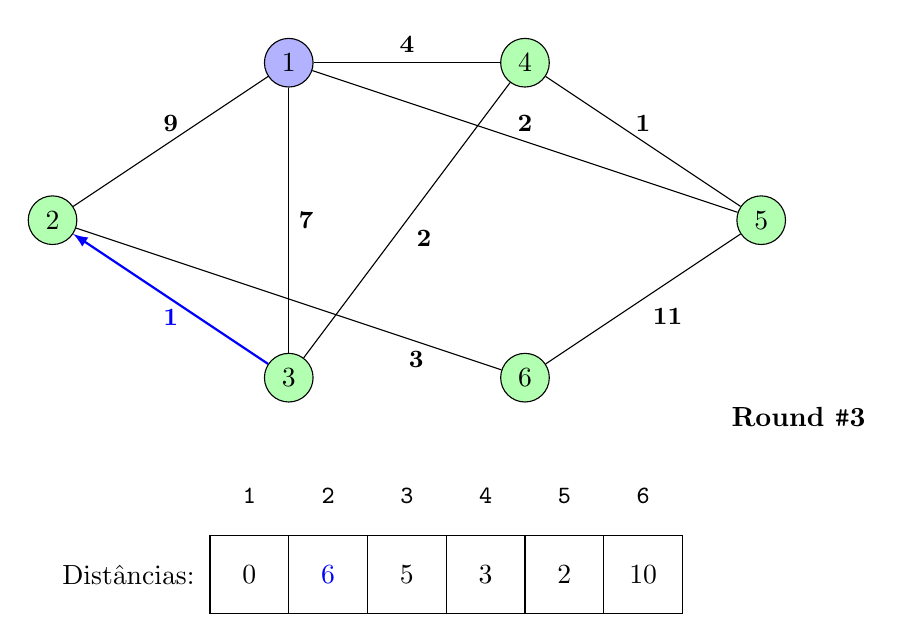
\begin{tikzpicture}
        \node[anchor=west] at (0, 0.5) { Distâncias: };
        \node[anchor=west] at (8.5, 2.5) { \bfseries Round \texttt{\#}3 };

        \node[circle, draw, fill=blue!30] (a) at (3, 7) {1};
        \node[circle, draw, fill=green!30] (b) at (0, 5) {2};
        \node[circle, draw, fill=green!30] (c) at (3, 3) {3};
        \node[circle, draw, fill=green!30] (d) at (6, 7) {4};
        \node[circle, draw, fill=green!30] (e) at (9, 5) {5};
        \node[circle, draw, fill=green!30] (f) at (6, 3) {6};

        \draw (2, 0) grid (8, 1);

        \node at (2.5, 0.5) { $0$ };
        \node at (3.5, 0.5) { \textcolor{blue}{$6$} };
        \node at (4.5, 0.5) { \textcolor{black}{$5$} };
        \node at (5.5, 0.5) { \textcolor{black}{$3$} };
        \node at (6.5, 0.5) { \textcolor{black}{$2$} };
        \node at (7.5, 0.5) { \textcolor{black}{$10$} };

        \node at (2.5, 1.5) { \small \texttt{1} };
        \node at (3.5, 1.5) { \small \texttt{2} };
        \node at (4.5, 1.5) { \small \texttt{3} };
        \node at (5.5, 1.5) { \small \texttt{4} };
        \node at (6.5, 1.5) { \small \texttt{5} };
        \node at (7.5, 1.5) { \small \texttt{6} };

        \draw (a) to node[midway,anchor=south] { \small \bfseries 9 } (b);
        \draw (a) to node[midway,anchor=west] { \small \bfseries 7 } (c);
        \draw (a) to node[midway,anchor=south] { \small \bfseries 4 } (d);
        \draw (a) to node[midway,anchor=south] { \small \bfseries 2 } (e);
        %\draw (b) to node[midway,anchor=north] { \small \bfseries 1 } (c);
        \draw[latex-,thick,blue] (b) to node[midway,anchor=north] { \small \bfseries 1 } (c);
        \draw (b) to node[pos=0.8,anchor=north] { \small \bfseries 3 } (f);
        \draw (c) to node[midway,anchor=north west] { \small \bfseries 2 } (d);
        \draw (d) to node[midway,anchor=south] { \small \bfseries 1 } (e);
        \draw (e) to node[midway,anchor=north west] { \small \bfseries 11 } (f);

    \end{tikzpicture}

\end{frame}

\begin{frame}[fragile]{Visualização do algoritmo de Bellman-Ford}

    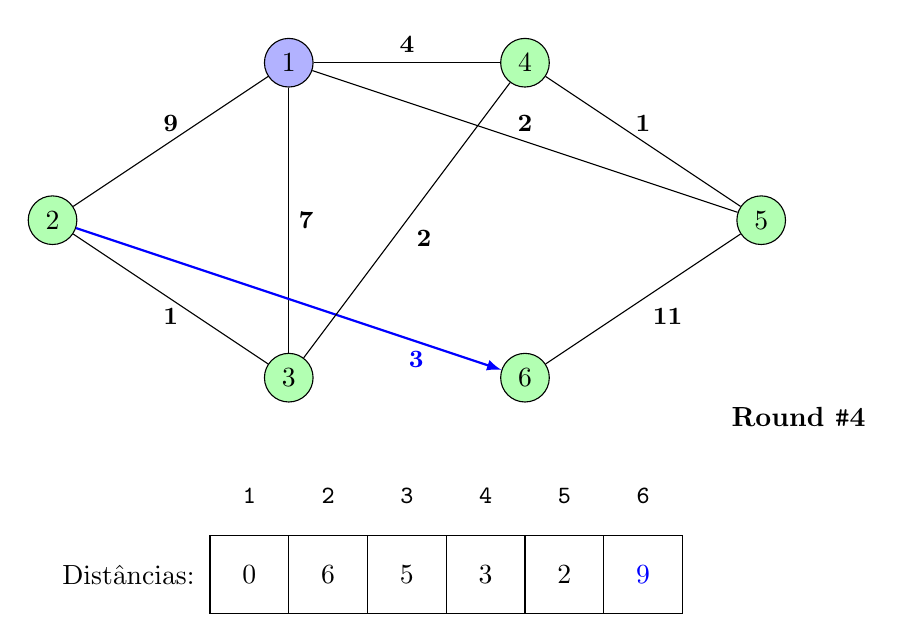
\begin{tikzpicture}
        \node[anchor=west] at (0, 0.5) { Distâncias: };
        \node[anchor=west] at (8.5, 2.5) { \bfseries Round \texttt{\#}4 };

        \node[circle, draw, fill=blue!30] (a) at (3, 7) {1};
        \node[circle, draw, fill=green!30] (b) at (0, 5) {2};
        \node[circle, draw, fill=green!30] (c) at (3, 3) {3};
        \node[circle, draw, fill=green!30] (d) at (6, 7) {4};
        \node[circle, draw, fill=green!30] (e) at (9, 5) {5};
        \node[circle, draw, fill=green!30] (f) at (6, 3) {6};

        \draw (2, 0) grid (8, 1);

        \node at (2.5, 0.5) { $0$ };
        \node at (3.5, 0.5) { \textcolor{black}{$6$} };
        \node at (4.5, 0.5) { \textcolor{black}{$5$} };
        \node at (5.5, 0.5) { \textcolor{black}{$3$} };
        \node at (6.5, 0.5) { \textcolor{black}{$2$} };
        \node at (7.5, 0.5) { \textcolor{blue}{$9$} };

        \node at (2.5, 1.5) { \small \texttt{1} };
        \node at (3.5, 1.5) { \small \texttt{2} };
        \node at (4.5, 1.5) { \small \texttt{3} };
        \node at (5.5, 1.5) { \small \texttt{4} };
        \node at (6.5, 1.5) { \small \texttt{5} };
        \node at (7.5, 1.5) { \small \texttt{6} };

        \draw (a) to node[midway,anchor=south] { \small \bfseries 9 } (b);
        \draw (a) to node[midway,anchor=west] { \small \bfseries 7 } (c);
        \draw (a) to node[midway,anchor=south] { \small \bfseries 4 } (d);
        \draw (a) to node[midway,anchor=south] { \small \bfseries 2 } (e);
        \draw (b) to node[midway,anchor=north] { \small \bfseries 1 } (c);
        %\draw (b) to node[pos=0.8,anchor=north] { \small \bfseries 3 } (f);
        \draw[-latex,thick,blue] (b) to node[pos=0.8,anchor=north] { \small \bfseries 3 } (f);
        \draw (c) to node[midway,anchor=north west] { \small \bfseries 2 } (d);
        \draw (d) to node[midway,anchor=south] { \small \bfseries 1 } (e);
        \draw (e) to node[midway,anchor=north west] { \small \bfseries 11 } (f);

    \end{tikzpicture}

\end{frame}


\begin{frame}[fragile]{Solução $O(NM)$}
    \inputsnippet{cpp}{1}{21}{codes/frete_bf.cpp}
\end{frame}

\begin{frame}[fragile]{Solução $O(NM)$}
    \inputsnippet{cpp}{22}{42}{codes/frete_bf.cpp}
\end{frame}

\begin{frame}[fragile]{Algoritmo de Dijkstra}

    \begin{itemize}
        \item Inicialmente, a distância de $s$ a $s$ é igual a zero, e todas as demais
            distâncias são iguais a infinito

        \item A cada iteração, o algoritmo escolhe o nó $u$ mais próximo de $s$ que ainda não foi
            processado

        \item Todas as arestas de partem de $u$ então são processadas, atualizando as 
            distâncias quando possível

        \item Esta operação de atualização de distância é chamada relaxamento

        \item Para escolher o próximo nó a ser processado de forma eficiente pode ser utilizada uma
            fila com prioridade

        \item Desta forma, a complexidade do algortimo é $O(N + M\log M)$

    \end{itemize}

\end{frame}

\input{dijkstra_view}

\begin{frame}[fragile]{Solução $O(N + M\log M)$}
    \inputsnippet{cpp}{1}{21}{codes/frete.cpp}
\end{frame}

\begin{frame}[fragile]{Solução $O(N + M\log M)$}
    \inputsnippet{cpp}{23}{43}{codes/frete.cpp}
\end{frame}

\begin{frame}[fragile]{Solução $O(N + M\log M)$}
    \inputsnippet{cpp}{45}{65}{codes/frete.cpp}
\end{frame}

\begin{frame}[fragile]{Solução $O(N + M\log M)$}
    \inputsnippet{cpp}{66}{86}{codes/frete.cpp}
\end{frame}
